\documentclass[a4paper, 10pt]{article}
\usepackage[unicode=true, colorlinks=true, linkcolor=blue, urlcolor=blue, citecolor=blue]{hyperref}
\usepackage[T2A]{fontenc}
\usepackage[utf8]{inputenc}
\usepackage[russian]{babel}
\usepackage{indentfirst}
\usepackage{amssymb}
\usepackage{enumitem}
\usepackage{hyperref}
\usepackage{geometry}
\usepackage{mathtools}
\usepackage{setspace}
\usepackage{tikz}
\usepackage{textcomp}
\usepackage{ stmaryrd }
\usepackage{ dsfont }
\usepackage{graphicx}
\graphicspath{{img/}}
\DeclareGraphicsExtensions{.pdf,.png,.jpg}
\usepackage{tikzsymbols}
\usepackage{upgreek}
\usepackage{ tipa }

\renewcommand{\C}{\mathbb{C}}
\newcommand{\N} {\mathbb{N}}
\newcommand{\Q} {\mathbb{Q}}
\newcommand{\Z} {\mathbb{Z}}
\newcommand{\R} {\mathbb{R}}

\renewcommand{\r}{\right}
\renewcommand{\l}{\left}

\geometry{a4paper,top=2cm,bottom=2cm,left=2cm,right=2cm}
\usepackage{hwspecial}


\title{Коллоквиум 2 по дискретной математике}
\author{Элбакян Сурен  \href{https://t.me/E7SSSS}{@E7SSSS}, \\ Артём Парфенов \href{https://t.me/dunno_0}{@dunno}, \\ Аксененко Вероника \href{https://t.me/akveronika}{@akveronika}}
\date{March 2022}


\begin{document}

\maketitle

\tableofcontents

\newpage

\section{Список определений и теорем из курса}

\subsection{Отношения эквивалентности. Классы эквивалентности.}

\textbf{Определение.} Бинарное отношение $R$ на множестве $X$ называется отношением эквивалентности, если выполнены следующие свойства:

\begin{itemize}
    \item (рефлексивность) $x R x \ \forall x \in X$
    \item (симметричность) $x R y \ \implies \ y R x \ \forall x,y \in X$
    \item (транзитивность) $x R y$ и $y R z \ \implies \ x R z \ \forall x, y, z \in X$
\end{itemize}

\textbf{Определение.} Любое отношение $R$, являющееся отношением эквивалентности на множестве $A$, делит $A$ на классы эквивалентности - непересекающиеся подмножества множества $A$, при этом любые два элемента одного класса находятся в отношении $R$, а любые два элемента разных классов не находятся в отношении $R$.

\subsection{Изоморфизм графов.}

\textbf{Определение.} Графы $G_1 = (V_1, E_1)$ и $G_2 = (V_2, E_2)$ называются изоморфными (обозначение $G_1 \cong G_2$), если существует такая биекция $\pi: V_1 \to V_2$ на множествах их вершин, которая переводит множество рёбер первого графа в множество рёбер второго графа, т.е. $\{u, v\} \in E_1$ равносильно $\{\pi(u), \pi(v)\} \in E_2$.

Неформально это определение можно пересказать так: графы изоморфны, если можно так отождествить их вершины, чтобы рёбра этих графов совпали.

\subsection{Инварианты изоморфизма, примеры.}

\textbf{Определение.} Изоморфизм сохраняет все свойства графов, которые выражаются в терминах связей между вершинами и рёбрами и не ссылаются на конкретные имена вершин. Такие свойства называются инвариантами изоморфизма.

\textbf{Примеры.} Например, число вершин в графе - инвариант изоморфизма, так как биекция возможна лишь между множествами одинакового размера.

Число рёбер в графе также является инвариантом изоморфизма, так как изоморфизм устанавливает взаимно однозначное соответствие между рёбрами.

Степень вершины сама по себе инвариантом изоморфизма не является. Но степень вершины сохраняется при изоморфизме: соседей у $v$ ровно столько же, сколько
у $\pi(v)$: соседи вершины обязаны переходить в соседей её образа.

\subsection{Отношения порядка: строгого, нестрогого.}

\textbf{Определение.} Бинарное отношение $R$ на множестве $X$ является строгим частичным порядком, если выполненые такие свойства:

\begin{itemize}
    \item (транзитивность) $xRy$ и $yRz \ \implies \ xRz \ \forall x, y, z \in X$
    \item (антирефлексивность) $xRx \equiv 0 \ \forall x \in X$
\end{itemize}

\textbf{Определение.} Бинарное отношение $\leqslant$ на множестве $X$ является нестрогим частичным порядком, если выполненые такие свойства:

\begin{itemize}
    \item (рефлексивность) $a \leqslant a \ \forall a \in X$
    \item (антисимметричность) $(a \leqslant b)$ и $(b \leqslant a) \ \implies \ (a = b) \ \forall a, b \in X$
    \item (транзитивность) $(a \leqslant b)$ и $(b \leqslant c) \ \implies \ (a \leqslant c) \ \forall a, b, c \in X $
\end{itemize}

\subsection{Покоординатное произведение частичных порядков.}

\textbf{Определение.}  Пусть $P, Q$ - два частичных порядка. Тогда покоординатный порядок на декартовом произведении $P \times Q$ задаётся правилом: $$(p_1, q_1) \leqslant (p_2, q_2) \text{ по определению означает } p_1 \leqslant_P p_2 \text{ и } q_1 \leqslant_Q q_2$$

\subsection{Лексикографическое произведение частичных порядков.}

\textbf{Определение.} Пусть $P, Q$ — два частичных порядка. Лексикографический порядок на $P \times Q$ задаётся правилом: $$(p_1, q_1) \leqslant (p_2, q_2) \text{ по определению означает } (p_1 <_P p_2) \text{ или } (p_1 = p_2) \text{ и } (q_1 \leqslant_Q q_2)$$

\subsection{Лексикографический порядок на словах.}

\textbf{Определение.} Пусть $A$ - линейно упорядоченное множество, скажем, множество двоичных цифр $0 < 1$, или множество десятичных цифр, или множество букв кириллического алфавита со стандартным порядком, задаваемым азбукой. На множестве слов в алфавите A, то есть конечных последовательностей элементов $A$, определим порядок правилом: если слово $x$ является началом слова $y$, то $x \leqslant y$. Если ни одно из слов $x, y$ не является началом другого, то найдётся позиция, в которой эти слова различаются. Тогда меньше то слово, в котором на этой позиции меньший символ алфавита.

\subsection{Изоморфизм порядков.}

\textbf{Определение.} Порядки $P$ и $Q$ называются изоморфными (обозначение $P \cong Q$), если есть такая биекция $\varphi: P \to Q$, что $x \leqslant y$ равносильно $\varphi(x) \leqslant \varphi(y)$ для всех пар $x, y$.

\subsection{Сумма частичных порядков.}

\textbf{Определение.} Пусть $P, Q$ — два частичных порядка, $P' \cong P$, $Q' \cong Q$, $P' \cap Q' = \varnothing$. Суммой $P + Q$ называется порядок на $P' \cup Q'$, в котором все элементы $P'$ меньше всех элементов $Q'$ , а пары элементы из $P'$ или $Q'$ сравниваются в порядках $P'$ и $Q'$ соответственно.

\subsection{Примеры неизоморфных линейных порядков на бесконечных множествах.}

Докажем, что $\NN + \ZZ$ и $\ZZ + \NN$ неизоморфны. Чтобы перейти к непересекающимся множествам, рассмотрим обычные целые числа и «штрихованные натуральные»: числа вида $0', 1', \dots$. Сравниваются эти числа так же, как нештрихованные. Но теперь множества не пересекаются (штрих либо есть, либо его нет).

В $\NN + \ZZ$ есть наименьший элемент - $0'$ меньше всех остальных элементов суммы порядков. А в $\ZZ + \NN$ такого элемента нет (для каждого целого числа есть меньшее его).

\subsection{Линейные порядки на конечных множествах.}
\textbf{Определение.} Линейный порядок - каждая пара элементов сравнима.

\textbf{Теорема.} Пусть $(X, \leqslant)$ и $(Y, \leqslant)$ - два линейных порядка на конечных множествах и $|X| = |Y|$. Тогда эти порядки изоморфны.

\textbf{Лемма.} В конечном линейном порядке есть наибольший и наименьший элементы.

\subsection{Теорема Дилуорса.}

\textbf{Определение.} Цепь - это такое подмножество частично упорядоченного множества, которое образует линейный порядок. Антицепь - это такое подмножество, в котором элементы попарно несравнимы.

\textbf{Теорема.} Наибольший размер антицепи в порядке равен наименьшему количеству цепей в разбиениях порядка на непересекающиеся цепи.

\subsection{Бесконечно убывающие цепи. Фундированные множества.}
\textbf{Определение.} Бесконечно убывающая цепь - бесконечная последовательность элементов порядка, что каждый следующий меньше предыдущего.

\textbf{Теорема.} Следующие свойства порядка $P$ равносильны: \\
1. каждое непустое подмножество имеет минимальный элемент; \\
2. любая убывающая цепь $y_1 > y_2 > y_3 > \dots$ конечна; \\
3. для порядка $P$ справедлив принцип индукции: если для утверждения $A(p)$, зависящего от элемента порядка, для любого $p$ верно утверждение «если $A(q)$ верно при всех $q < p$, то и $A(p)$ верно». Тогда утверждение $A(p)$ верно при любом $p \in P$ .

\textbf{Определение.} Порядок, удовлетворяющий условиям теоремы , называется фундированным. Множество с фундированным порядком для краткости также называется фундированным.

\subsection{Принцип математической индукции для фундированных множеств}

Напомним принцип полной математической индукции: \\

Пусть для последовательности утверждений $$A_1, A_2, A_3, \dots , A_n, \dots$$ занумерованных целыми положительными числами, истинно утверждение: «для любого $n$ из истинности $A_i$ при всех $i < n$ следует истинность $A_n$». Тогда $A_n$ истинно для любого $n$ \\

Здесь используется порядок на натуральных числа. Однако аналогичное утверждение справедливо для более широкого класса порядков.

Мы также формулировали принцип наименьшего числа $$\text{
Любое непустое подмножество натуральных чисел содержит наименьший элемент.}$$

Здесь также используется порядок на натуральных числах. Для обобщения индукции нужны не наименьшие, а минимальные элементы порядков. Разница существенная: наименьший элемент меньше или равен всякого элемента порядка, а минимальный обладает более слабым свойством: нет элементов, которые меньше минимального. Скажем, в антицепи нет наименьшего элемента, но всякий элемент антицепи - минимальный.

\subsection{Общая формула включений-исключений.}

\textbf{Теорема(Формула включений и исключений).} %$$\includegraphics{включения-исключения.png}$$

\medskip

$|A_1 \cup A_2 \cup \dots \cup A_n| = |A_1| + \dots + |A_n| - $

$- |A_1 \cap A_2| - |A_1 \cap A_3| - \dots $

$+ |A_1 \cap A_2 \cap A_3| + |A_1 \cap A_2 \cap A_4| + \dots$

$\dots$

$+ (-1)^{n + 1} |A_1 \cap A_2 \cap \dots \cap A_n|$

\medskip

В первой строчке правой части равенства выписаны мощности всех множеств. Во второй — мощности всех попарных пересечений множеств (со знаком минус). Далее выписываем пересечения троек, четвёрок и т.д. множеств с чередующимися знаками.

\subsection{Подсчет монотонных путей по прямой, рекуррентные формулы для разных случаев.}

Есть клетчатая лента, по которой можно двигать фишку. Клетки пронумерованы целыми числами. В начале фишка находится в клетке 0. Далее её можно сдвигать вправо. Нужно подсчитать, сколько есть различных способов попасть в клетку с номером $n$.

\textbf{Пример.} Пусть разрешены ходы на одну и на две клетки.

Тогда, если  количество таких способов $F_n$, то $F_{n + 2} = F_{n+1} + F_n$

\textbf{Пример.} Пусть разрешены ходы на любое количество клеток.

Тогда, если количество таких способов $T(n)$, то $T(n) = T(n - 1) + T(n - 2) + \dots + T(0) = 2 \cdot T(n - 1)$

\subsection{Формула произведения. Подсчёт слов длины $n$ в конечном алфавите.}

\textbf{Правило произведения.} Для конечных множеств $A, B$ выполняется равенство $|A \times B| = |A| \cdot |B|$(в общем случае, $|A_1 \times A_2 \times \dots \times A_n| = |A_1| \cdot |A_2| \cdot \dots \cdot |A_n|$)

\textbf{Пример.} Подсчитаем количество слов длины $n$ в алфавите $A$ из $k$ символов. По определению, слово - это последовательность $a_1 \dots a_n$, где $a_i \in A$. Другими словами, множество слов длины n - это декартова степень $A^n$. По формуле произведения получаем, что количество слов равно $k^n$. В частном случае $k = 2$ мы уже получали эту формулу: двоичных слов длины $n$ ровно $2^n$ штук.

\subsection{Размещения и упорядоченные выборки.}

\textbf{Определение.Размещение(упорядоченные выборки)} Размещение из k по n — это слово длины n в алфавите из k символов, в котором все символы разные.

$A_{k, n + 1} = (k - n)A_{k, n}$

$A_{k, n} = k(k - 1)(k - 2) \cdot \dots \cdot (k - n + 1) = \cfrac{k!}{(k - n)!}$

\subsection{Сочетания из $n$ по $k$}

\textbf{Определение.} Сочетание из $n$ элементов по $k$ - подмножество $n$-элементного множества, в котором ровно $k$ элементов. $$C^k_n = \frac{n!}{k!(n - k)!}$$

\subsection{Биномиальные и мультиномиальные коэффиценты.}

Рассмотрим бином $(x + y)^n$. Как известно из алгебры, целое алгебраическое выражение можно записать в виде многочлена. Поэтому $$(x + y)^n = \sum^n_{k = 0} \binom{n}{k}x^{k}y^{n - k}\text{, где} \binom{n}{k} = C^k_n = \frac{n!}{k!(n - k)!}$$

Используем следующую запись: моном $x_1^{a_1}x_2^{a_2} \dots x_k^{a_k}$ однозначно определяется последовательностью показателей $\alpha =
(a_1, a_2, \dots , a_k)$, мы будем обозначать такой моном сокращённо как $x^{\alpha}$. Разложение $$(x_1 + x_2 + \dots + x_k)^n = \sum_{\alpha}\binom{n}{\alpha}x^{\alpha} \text{, где } \binom{n}{a_1, a_2, \dots , a_k} = \frac{n!}{a_1!a_2! \dots a_k!}$$

\subsection{Монотонные пути в целочисленном квадранте. Формула. Треугольник Паскаля}

Рассматриваем монотонные пути на плоскости. Мы двигаем фишку по точкам плоскости с целыми координатами. За один шаг можно увеличить абсциссу на 1 или ординату на 1. Сколько есть различных монотонных путей из точки $(0, 0)$ в точку $(a, b)$? Обозначим это количество $T(a, b)$.

\medskip

Формуля для $T$:

1)$T(a, b) = T(a - 1, b) + T(a, b - 1)$

2)$T(a, b) = \binom{a + b}{a} = \frac{(a+b)!}{a!b!}$

\medskip

Биномиальные коэффициенты часто записывают в виде треугольника Паскаля: \\
%$$\includegraphics{PascalTriangle.png}$$

$${\centering \begin{array}{c}
	1 \\
	1 \quad 1 \\
	1 \quad 2 \quad 1 \\
	1 \quad 3 \quad 3 \quad 1 \\
	1 \quad 4 \quad 6 \quad 4 \quad 1 \\
	1 \quad 5 \quad 10 \quad 10 \quad 5 \quad 1 \\
	1 \quad 6 \quad 15 \quad 20 \quad 15 \quad 6 \quad 1 \\
	1 \quad 7 \quad 21 \quad 35 \quad 35 \quad 21 \quad 7 \quad 1 \\
\end{array}}$$

\subsection{Свойства биномиальных коэффицентов и чисел в треугольнике Паскаля.}

\textbf{Утверждение.} Каждая строка треугольника Паскаля симметрична относительно середины.

\textbf{Утверждение.} В первой половине строки треугольника Паскаля числа возрастают.

\textbf{Утверждение.} Каждое число в треугольнике Паскаля по крайней мере в 2 раза меньше, чем число, которое стоит под ним.

\textbf{Утверждение.} Количество подмножеств n-элементного множества с нечётным количеством элементов равно количеству подмножеств n-элементного множества с чётным количеством элементов.
\subsection{Подсчёт функций из конечного множества в конечное: формулы для количества всех функций, тотальных, инъекций, сюръекций, биекций}

Подсчитаем количество тотальных функций из конечного $n$ - элементного множества $A$ в конечное $k$ - элементное множество $B$.

\textbf{Тотальных функций - } $k^n$

\textbf{Всего функций - } $(k + 1)^n$

\textbf{Инъекций - } $\cfrac{k!}{(k - n)!}$

\textbf{Сюръекций - } $\sum^{k}_{p=0}(-1)^p \binom{k}{p} (k - p)^n = k^n - \sum^{n}_{p=1}(-1)^{p+1} \binom{k}{p}(k - p)^n$

\textbf{Биекций - } $n!$

\subsection{Сочетания с повторениями из $n$ по $k$. Формула.}

Моном $x^{a_1}x^{a_2} \dots x^{a_n}$ имеет степень $a_1 + \dots + a_n$ и
мономы совпадают тогда и только тогда, когда соответствующие последовательности показателей равны. Поэтому нам нужно найти количество решений уравнения
$$a_1 + \dots + a_n = k$$
в неотрицательных целых числах. Количество мономов степени $k$ традиционно называется числом сочетаний с повторениями из n по k. Обозначим его $$\left(\binom{n}{k} \right)$$

\textbf{Формула.} $\left(\binom{n}{k} \right) = \binom{n + k - 1}{k}$

\subsection{Числа Каталана.}

\textbf{Определение.} Двигаем фишку по целочисленным точкам треугольника $x \geqslant 0, y \geqslant 0, x \geqslant y$. На каждом шаге можно увеличить одну из координат на 1. Количество таких монотонных путей внутри треугольника из точки $(0, 0)$ в точку $(n, n)$ обозначается $C_n$ и называется $n$-м числом Каталана.

\textbf{Теорема.} $C_n = \frac{1}{2n+1} \binom{2n+1}{n} = \frac{1}{n+1} \binom{2n}{n}$

\subsection{Элементарная теория вероятностей: конечное множество исходов, вероятности исходов, вероятностное пространство, события, вероятность события}

\textbf{Определение.} Вероятностное пространство - конечное множество $U$, его элементы называются возможными исходами.

\textbf{Определение} Функция $Pr : U \to [0, 1]$, удовлетворяющая соотношению $\sum_{x \in U}Pr[x] = 1$, называется вероятностным распределением, а число $Pr[x]$ называется вероятностью исхода $x \in U$.

\textbf{Определение.} Событием называется произвольное подмножество $A \subseteq U$.

\textbf{Определение.} Вероятностью события $A$ называется число $Pr[A] = \sum_{x \in A} Pr[x]$

\subsection{Равномерное распределение. Примеры: подбрасывания монеты, подбрасывания игральной кости, случайные перестановки.}

В модели с равновозможными исходами функция $Pr$ задаётся формулой $Pr[x] = 1/|U|$ для всякого $x \in U$($U$ -  вероятностное пространство)(такое распределение называют также равномерным).

\textbf{Пример(«Подбрасывание монеты»).} В случае подбрасывания монетки исходом является выпадение одной из её сторон, орла или решки. Всего исходов, таким образом, два, и они считаются равновозможными. Обычно удобнее говорить не о сторонах монетки, а отождествить их с числами 0 и 1.
Итак, вероятностное пространство: числа 0 и 1. Все исходы равновозможны.

\textbf{Пример(«Подбрасывание n монет»).} Вероятностное пространство: двоичные слова длины $n$. Все слова равновозможны. Какова вероятность события «на $i$-й позиции в слове стоит 1»?\\
Всего исходов $2^n$ (количество двоичных слов длины $n$). Интересующее нас событие содержит $2^{n-1}$ исходов: каждый такой исход задаётся выбором 0 или 1 для всех позиций кроме $i$-й. Вероятность этого события равна по определению $2^{n-1} / 2^n = 1/2$, как и вероятность дополнительного события «на $i$-й позиции в слове стоит 0».

\textbf{Пример(«Случайная перестановка»).} Это случай выборки без возвращения при k = n. Вероятностное пространство: перестановки $(a_1, a_2, \dots , a_n)$ чисел от $1$ до $n$. Все исходы равновозможны. \\
Посчитаем вероятность события $a_1 = 1$. Благоприятные исходы образуют множество перестановок, в которых 1 стоит на первом месте. Остальные элементы стоят как угодно, поэтому благоприятные исходы находятся во взаимно однозначном соответствии с перестановками $n - 1$ элемента. Вероятность равна $(n - 1)!/n! = 1/n$. \\
Вероятность события $a_n = 1$ такая же. Теперь благоприятные исходы образуют множество перестановок, в которых 1 стоит на последнем месте. И в этом случае благоприятные исходы находятся во взаимно однозначном соответствии с перестановками $n - 1$ элемента.


\subsection{Несовместные и дополнительные события. Суммы вероятностей.}
Дополнительное событие $\overline{A}$ это просто разность $U \setminus A$. Легко увидеть из определения распределения вероятностей, что всегда $Pr[A] + Pr[\overline{A}] = 1$

События A и B, которые не могут произойти одновременно, то есть для которых $Pr[A \cap B] = 0$, называются несовместными.

\subsection{Оценка объединения.}

\textbf{Лемма.} Если события $A_i$ попарно несовместны, то $$Pr[\bigcup^{n}_{i=1}A_i] = \sum^{n}_{i=1}Pr[A_i]$$

\textbf{Лемма(оценка объединения).} Для любых событий $A_1, \dots , A_n \subseteq U$ выполняется неравенство $$Pr[\bigcup^{n}_{i=1}A_i] \leqslant \sum^{n}_{i=1}Pr[A_i]$$

\subsection{Вероятностный метод. Существование графов Рамсея.}

\textbf{Лемма(«среднее не больше максимума и не меньше минимума»).} Пусть $\mathbb{E}[f] = C$ для какой-то случайной величины $f : U \to \RR$. Тогда существует такой исход $u \in U$, что верно $f(u) \geqslant C$. Аналогично, существует и такой исход $u \in U$, что $f(u) \leqslant C$.

\textbf{Теорема.} $R(k,k) \geqslant \lfloor 2^{(k-1)/2} \rfloor$ при всех $k \geqslant 3$. Другими словами, для всякого $k \geqslant 3$ существует граф $G = (V,E)$ на $n = \lfloor 2^{(k-1)/2} \rfloor$ вершинах, в котором нет ни клики размера $k$, ни независимого множества размера $k$.


\subsection{Формула включений и исключений для вероятностей.}

%$$\includegraphics{вкл_искл.png}$$

\textbf{Теорема. Для всякой вероятностной модели и для произвольных множеств $A_1, \dots A_n \subseteq U$ верно}

$$\Huge Pr[A_1 \cup A_2 \cup \dots \cup A_n] = \sum_i Pr[A_i] - \sum_{i < j} Pr[A_i \cap A_j] + \dots = \sum_{\varnothing \neq S \subset \{1, 2, \dots, n\}} (-1)^{|S| + 1} Pr[\cap_{i \in S} A_i]$$

\subsection{Задача о беспорядках.}

\textbf{Лемма}

Рассмотрим случайные перестановки n различных объектов, то есть рассмотрим вероятностное пространство всех перестановок n заданных объектов, причём в перестановки равновозможны. Пусть $A_n$ - событие означающее, что все объекты после перестановки оказались не на своих местах.

Тогда $\lim \limits_{n \to +\infty} Pr[A_n] = \frac{1}{e}$

\textbf{Доказательство.}

Зафиксируем n и обозначим через $B_i$, где $i = 1, \dots, n$, событие «объект с номером i остался на месте». Тогда $\cup_{i} B_i$ означает, что хотя бы один из элементов остался на месте. Дополнительное к этому событие - как раз искомо $A_n$.

Применим формулу включений-исключений к $\cup_{i} B_i$. Для этого нам нужно посчитать вероятности событий $\cap_{i} B_i$ для всех $S \subseteq [n]$. Перестановки из этого события - это в точности перестановки, оставляющие на месте элементы из $S$, и переставляющие остальные элементы произвольным образом. Таких перестановок $(n - |S|)!$ Таким образом, $\forall S$

$$Pr[\cap_{i} B_i] = \frac{(n - |S|)!}{n!}$$

Множеств $S$ размера $k$ всего $C_n^k$, так что по формуле включений-исключений получим

$$Pr[\cup_{i} B_i] = \sum_{k = 1}^n (-1)^{k + 1} C_n^k \cdot \frac{(n - k)!}{n!} = \sum_{k = 1}^n (-1)^{k + 1} \frac{1}{k!}$$

Тогда для вероятности $A_n$ получаем формулу

$$Pr[A_n] = 1 - \sum_{k = 1}^n (-1)^{k + 1} \frac{1}{k!} = \sum_{k = 0}^n \frac{(-1)^k}{k!}$$

Что совпадает с началом ряда Тейлора для $e^x$ в т. $x = -1$. Т.к. $e^{-1} = \sum_{k=0}^\infty \frac{(-1)^k}{k!}$, то

$$\lim \limits_{n \to +\infty} Pr[A_n] = \frac{1}{e}$$

$\hfill \blacksquare$

\subsection{Условная вероятность, цепное правило для вероятности пересечения событий. Примеры вычисления условных вероятностей.}

\textbf{Определение.} Условной вероятностью события $A$ при условии события $B$ называется число $$Pr[A|B] = \cfrac{Pr[A \cap B]}{Pr[B]}$$

\textbf{Следствие.} $Pr[A \cap B] = Pr[B] \cdot Pr[A|B]$

\textbf{Примеры.}  В урне находятся 3 белых шара и 2 черных. Из урны вынимается один шар, а затем второй. Событие В – появление белого шара при первом вынимании. Событие А – появление белого шара при втором вынимании.

$Pr[A|B] = \cfrac{Pr[A \cap B]}{Pr[B]}$ очевидно, что $Pr[A \cap B] = \frac{3}{5} \cdot \frac{2}{4}$ и $Pr[B] = \frac{3}{5}$ $\to$ $Pr[A|B] = \frac{1}{2}$

\subsection{Определение независимых событий. Примеры проверки независимости событий.}

\textbf{Определение.} Событие $A$ не зависит от события $B$, если $Pr[A] = Pr[A|B]$, что эквивалентно(выводится из формулы условной вероятности) $Pr[A \cap B] = Pr[B] \cdot Pr[A]$

\textbf{Примеры.} Пусть два раза подбрасывают игральную кость. Событие $A$ = «при броске выпало четное число» и $B$ = «при втором броске выпало четное число». Зависимы ли события $A$ и $B$?

$Pr[A] = Pr[B] = 3/6 = 1/2$, $Pr[A \cap B] = 9/36 = 1/4$(так как на первом броске может выпасть 1 из 3 четных чисел, и на втором броске 1 из 3), заметим, что $Pr[A \cap B] = Pr[B] \cdot Pr[A]$ $\to$ события независимы.

\subsection{Формула Байеса.}

\textbf{Лемма(формула Байеса).} Если вероятности событий $A$ и $B$ положительны, то $$Pr[A|B] = Pr[A] \cdot \cfrac{Pr[B|A]}{Pr[B]}$$

\subsection{Формула полной вероятности. Примеры использования.}

\textbf{Лемма(формула полной вероятности).} Пусть $B_1, \dots, B_n$ - разбиение вероятностного пространства $U$, то есть $U = B_1 \cup \dots \cup B_n$, где $B_i \cap B_j = \varnothing$ при $i \neq j$. Пусть также $Pr[B_i] > 0$ для всякого $i$. Тогда для всякого события $A$ $$Pr[A] = \sum^n_{i = 1}Pr[A|B_i] \cdot Pr[B_i]$$

\textbf{Пример.} Болезнью К больны 1\% людей в городе М. Тест П даёт положительный результат для 99\% больных и для 1\% здоровых. Я сдал тест и тот оказался положительным. Какова вероятность, что я болен? \\
События, о которых идёт речь: A = болен, B = тест дал положительный результат. Из данных о тесте мы знаем, что $Pr[B|A] = 0.99$. Вероятность $Pr[A]$ равна 0.01. Чтобы найти $Pr[B]$, нужно использовать формулу полной вероятности: \\
$Pr[B] = Pr[A] \cdot Pr[B|\text{болен}] + Pr[\overline{A}] \cdot Pr[B|\text{здоров}] = 0.01 \cdot 0.99 + 0.99 \cdot 0.01 = 0.0198$ \\
По формуле Байеса получаем ответ: $Pr[A|B] = 0.01 \cdot 0.99/0.0198 = 0.5$

\subsection{Определение случайной величины и математического ожидания.}

Случайная величина - это числовая функция на вероятностном пространстве, то есть функция вида $f : U \to R$.

Важным параметром случайной величины является её математическое ожидание. Неформально, это число, которое мы будем получать в среднем, если повторять эксперимент много раз и каждый раз смотреть на значение случайной величины.

Формальное определение: математическим ожиданием случайной величины $f : U \to R$ называется число $$\mathbb{E}[f] = \sum_{x \in U}f(x)Pr[x]$$

\subsection{Линейность матожидания. Примеры использования.}

\textbf{Лемма.} Пусть $f : U \to R$ и $g : U \to R$ - две случайные величины на одном и том же вероятностном пространстве. Тогда $$\mathbb{E}[f + g] = \mathbb{E}[f] + \mathbb{E}[g]$$

\textbf{Пример.} Как пример можем привести задачку из дз
\begin{problem}{2}
Магазин назначил за каждый товар целую цену, а при покупке добавляет равновероятно к цене товару случайное число копеек (от 0 до 99). Покупатель взял 20 разных товаров и направился к кассе. Найдите математическое ожидание доплаты покупателя — разности между итоговой суммой к оплате и суммой к оплате без добавленных копеек.
\end{problem}
Рассмотрим случайная величину S - переплаченная сумма. Введем функцию случайную величину $\xi_i$ равную доплате за i товар. $S = \sum^{20}_{i=1} \xi_i$. Тогда $E[S] = E[\sum^{20}_{i=1} \xi_i] = \sum^{20}_{i=1} E[\xi_i] = \sum^{20}_{i=1} \sum^{99}_{\xi = 0} \xi \cdot P[\xi]$. В силу равновероятности выбора наценки $P[\xi] = \frac{1}{100}$. Нехитрыми мат. преобразованиями получаем $\sum^{20}_{i=1} \sum^{99}_{\xi = 0} \xi \cdot P[\xi] = \sum^{20}_{i=1} \frac{99}{2} = 990$.

\subsection{Неравенство Маркова. Примеры использования.}

\textbf{Лемма(неравенство Маркова).} Пусть $f$ - случайня величина, принимающая только неотрицательные значения. Тогда для всяего $\alpha > 0$ верно $$Pr[f \geqslant \alpha] \leqslant \cfrac{\mathbb{E}[f]}{\alpha}$$

\begin{problem}{1}
 В лотерее на выигрыши уходит 25\% от стоимости проданных билетов. Каждый билет стоит 40 рублей. Докажите, что вероятность выиграть не менее 1000 рублей не больше 1\%.
\end{problem}

Пусть A - случайная величина равная величине выигрыша, тогда $E[A] = 10$(нетрудно понять, что если отправляют 25\% от проданных билетов, то мат.ожидание выигрыша составляет 25\% от суммы проданны билетов). По неравенству Маркова имеем $P[A \geqslant 1000] \leqslant \cfrac{E[A]}{1000}$ $\to$ $P[A \geqslant 1000] \leqslant \cfrac{1}{100}$, что и требовалось доказать.

\subsection{Дисперсия, неотрицательность дисперсии.}

\textbf{Определение.} Дисперсия - мера разброса значений случайной величины относительно её математического ожидания $$\mathbb{D}[f] = \mathbb{E}[(f - E[f ])^2] = \mathbb{E}[f^2] - \mathbb{E}[f]^2$$


Так как математическое ожидание неотрицательной величины неотрицательно, дисперсия всегда неотрицательна. Дисперсия может равняться нулю. Что это означает? Если событие $f \neq \mathbb{E}[f]$ имеет положительную вероятность, то дисперсия заведомо положительная. Значит, $\mathbb{D}[f] = 0$ означает, что с вероятностью 1 величина $f$ принимает одно и то же значение.

\subsection{Неравенство Чёбышева.}

В общем случае дисперсия позволяет оценивать вероятность отклонения случайной величины от среднего (от математического ожидания).

\textbf{Лемма(Неравенство Чёбышева).} $Pr \left [|f - \mathbb{E}[f]| \geqslant \alpha \right] \leqslant \cfrac{\mathbb{D}[f]}{\alpha^2}$

\subsection{Независимость случайных величин.}

\textbf{Определение.} Величины $f, g$ назовём независимыми, если для любых $x, y$ события $f = x$ и $g = y$ независимы.

\textbf{Лемма.} Если $f, g$ независимы, то $\mathbb{E}[f \cdot g] = \mathbb{E}[f] \cdot \mathbb{E}[g]$

\subsection{Уклонения от среднего. Неравенство Хёфдинга-Чернова.}

\textbf{Определение.} Уклонение от среднего - разность значения случайной величины и ее математического ожидания.

Обозначим через $X_n$ случайную величину, равную количеству выпавших орлов после $n$ подбрасываний «честной» монеты, а через $\xi_n = X_n/n$ - частоту выпавших орлов. При больших n частота с очень большой вероятностью оказывается близкой к $1/2$. Имеет место следующая оценка, которая очень удобна в приложениях вероятностного метода в комбинаторике, а также в теоретической информатике.

\textbf{Теорема}(неравенство Хёфдинга-Чернова) $$Pr[|X_n - \frac{n}{2}| >  \epsilon n] = Pr[|\xi_n - \frac{1}{2}| > \epsilon] < 2e^{-2\epsilon^{2}n}$$

\subsection{Делимость целых чисел, основные свойства. Порядок делимости, простые числа.}

Деление (операция, обратная к умножению) не всегда возможно, если ограничиваться только целыми числами. Например, уравнение $2x = 1$ не имеет решений в целых числах.

\textbf{Определение.} Целое число $a$ делится на целое число $b$, если $a = bk$ для некоторого целого числа $k$. В этом случае говорят также «a кратно b», и «b является делителем числа a».

\textbf{Свойства.} \\
1. Все целые числа делятся на единицу. \\
2. Каждое целое число, не равное нулю, делится на натуральное число, равное модулю от данного целого. \\
3. Все натуральные числа являются делителями нуля. \\
4. Если целое число $a$ делится на натуральное число $b$ и модуль числа $a$ меньше $b$, то a равно нулю. \\
5. Если целое число $a$ отлично от нуля и делится на натуральное число $b$, то модуль числа $a$ не меньше числа $b$. \\
6. Единственный делитель единицы — сама единица. \\
7. Чтобы целое число $a$ делилось на натуральное число $b$, необходимо и достаточно, чтобы модуль числа $a$ делился на $b$. \\
8. Если натуральные числа делятся друг на друга без остатка, то они равны. \\

Получаем бинарное отношение на множестве целых чисел (иногда будем ограничивать его на множество положительных целых чисел). Принятое в современных математических книгах обозначение этого отношения $b | a$ (первое число - делитель второго, второе - кратное первого.

Отношение делимости $a | b$ является отношением нестрогого частичного порядка на положительных целых числах (будем обозначать это множество $\NN_+$). Антисимметричность: если $a | b$ и $b | a$, то $a = kb = kla$, откуда получаем $kl = 1$, то есть $k = l = 1$. Транзитивность: если $c = kb$ и $b = la$, то $c = kla$.

\textbf{Определение.} Целое положительное число называется простым, если оно больше 1 и делится только на 1 и на само себя.



\subsection{Деление с остатком: определение, примеры. Основные свойства.}

\textbf{Определение.} Разделить целое $a$ на целое положительное b означает найти такое целое $q$ (частное) и такое целое $r$ (остаток), что
$$a = b \cdot q + r; 0 \leqslant r < b$$

\textbf{Пример.} Остаток от деления 2022 на 100 равен 22, так как $2020 = 20 \cdot 100 + 22$. Остаток от деления -5 на 7 равен 2: $-5 = (-1) \cdot 7 + 2$.

\textbf{Свойства.} Деление с остатком всегда возможно, притом единственным
образом.

\subsection{Сравнения по модулю и равенство вычетов. Арифметические операции с вычетами.}

\textbf{Определение.} Если два числа $a$ и $b$ дают одинаковые остатки при делении на положительное число $N$, то говорят, что они сравнимы по модулю $N$, и пишут $a \equiv b$ (mod $N$).

Для любого N отношение сравнимости по модулю N является отношением эквивалентности. Классы эквивалентности — множества чисел, имеющих одинаковый остаток от деления на N, — называются классами вычетов или просто вычетами по модулю N.

\textbf{Пример.} Числа $\dots , -11, -5, 1, 7, \dots$ дают остаток 1 по модулю 6. Они образуют класс вычетов по модулю 6.

Когда мы говорим о вычете 1 по модулю 6, то имеем в виду всё это множество чисел.

\textbf{Арифметические операции с вычетами.} \\
$\{a+kN : k \in \ZZ \} + \{b + kN : k \in \ZZ\}= \{a + b + kN : k \in \ZZ \}$; \\
$\{ a + kN : k \in \ZZ\} \cdot \{b + kN : k \in \ZZ\} = \{ab+kN : k \in \ZZ\}$.

\textbf{Пример.} Теперь легко обосновать, почему остаток от деления $10^{10001}$ на 11 равен 10: $10^{10001} \equiv (-1)^{10001} = -1 \equiv 10$ (mod 11).

\subsection{Признаки делимости}

\textbf{Деление на 2.}Число a = $\overline{a_ka_{k-1}\dots a_0}$ делится на 2 тогда и только тогда, когда последняя цифра $a_0$ четна.

\textbf{Деление на 3.}Число a = $\overline{a_ka_{k-1}\dots a_0}$ делится на 3 тогда и только тогда, когда cумма его цифр делится на 3.

\textbf{Деление на 4.}Число a = $\overline{a_ka_{k-1}\dots a_0}$ делится на 4 тогда и только тогда, когда число, составленное из двух последних цифр, делится на 4.

\textbf{Деление на 5.}Число a = $\overline{a_ka_{k-1}\dots a_0}$ делится на 5 тогда и только тогда, когда последняя цифра $a_0$ делится на 5.

\textbf{Деление на 9.}Число a = $\overline{a_ka_{k-1}\dots a_0}$ делится на 9 тогда и только тогда, когда cумма его цифр делится на 9.

\textbf{Деление на 11.}Число a = $\overline{a_ka_{k-1}\dots a_0}$ делится на 11, если и только если знакопеременная сумма его цифр делится на 11.

\subsection{Свойства арифметики остатков}
Для каждого N определены сложение и умножение вычетов по модулю N. В силу леммы эти операции наследуют обычные свойства арифметических операций: \\
1)$a + (b + c) = (a + b) + c$ (ассоциативность сложения) \\
2)$ab = ba$ (коммутативность умножения) \\
3)$a(bc) = (ab)c$ (ассоциативность умножения) \\
4)$a(b + c) = ab + ac$ (дистрибутивность)

Числа 0 и 1 (точнее, классы вычетов, содержащие 0 и 1) при делении на N обладают обычными свойствами: \\
1)$0+a=a$ \\
2)$1 \cdot a=a$ \\
3)$0 \cdot a=0$

\subsection{Обратимые вычеты по модулю N. Критерий обратимости}
\textbf{Определение}. Вычет по модулю N называется обратимым, если в произведении с каким-то другим вычетом он даёт 1. Другими словами, a обратим, если уравнение $ax = 1$ имеет решение в арифметике вычетов.

\textbf{Критерий.} Обратимыми по модулю N являются те и только те вычеты, которые взаимно просты с N.

\subsection{Взаимно простые числа}
\textbf{Определение.} Взаимно простыми называются числа, которые не имеют общего положительного делителя, не считая 1.

\subsection{НОД и НОК, основные свойства.}

\textbf{Определение.} Наибольшим общим делителем $d$ для двух целых чисел $a$ и $b$ называется наибольший из их общих делителей, т.е. любой общий делитель $d'$ чисел $a, b$ является делителем числа $d$.

\textbf{Лемма.} НОД$(a, b)$ = НОД$(a - qb, b)$ для любого целого $q$.

\textbf{Определение.}НОК двух целых чисел $a$ и $b$ есть наименьшее натуральное число, которое делится на $a$ и $b$ без остатка, то есть кратно им обоим.

\textbf{Следствие.} НОД$(n, k) \cdot$НОК$(n, k) = kn$

\subsection{Количество решений линейного сравнения в вычетах.}

\textbf{Утверждение.} Сравнение $ax \equiv b$ (mod n) либо не имеет решений, если НОД$(a, n) \nmid b$, либо имеет ровно НОД$(a, n)$ решений в вычетах.

\subsection{Линейные диофантовы уравнения. Общая формула.}

\textbf{Определение.} Уравнение $$ax + by = c,$$ где $a, b, c$ - целые числа, называется линейным диофантовым уравнением.

\textbf{Теорема.} Пусть НОД$(a, b) | c$, $a\overline{x_0} + b\overline{y_0} = c$. Тогда множество решений уравнения $ax + by = c$ - это множество пар $$(\overline{x_0} + tb/\text{НОД}(a, b), \overline{y_0} - ta/\text{НОД}(a, b)), t \in \ZZ$$

\subsection{Однозначность разложения на простые делители}

\textbf{Теорема(Основная теорема арифметики).} Всякое целое положительное число, большее 1, разлагается на простые множители, причём единственным образом: любые два разложения отличаются только перестановкой сомножителей.

\subsection{Малая теорема Ферма}

\textbf{Теорема} Если p — простое число, то \\
$$a^{p-1} \equiv 1 \text{(mod p)}$$
при любом a, не делящемся на p.

\subsection{Функция Эйлера. Теорема Эйлера.}
\textbf{Определение.} Функция Эйлера $\varphi(n)$ равна количеству остатков по модулю n, взаимно простых с n.

\textbf{Теорема.} Пусть $n > 1$ — произвольное целое положительное число, $a$ взаимно прост с $n$. Тогда
$$a^{\varphi(n)} \equiv 1 \text{(mod n)}$$

\subsection{Китайская теорема}
\textbf{Теорема.} Пусть числа $u и v$ взаимно просты, и пусть $a$ и $b$ — любые целые числа. Тогда можно найти число $x$, для которого $x \equiv a$ (mod $u$) и одновременно $x \equiv b$ (mod $v$). В промежутке от 0 до $uv - 1$ такое число единственное.

\subsection{Мультипликативность функции Эйлера}

\textbf{Теорема(мультипликативность функции Эйлера).} $\varphi(uv) = \varphi(u)\varphi(v)$, если $u$ и $v$ взаимно просты.

\textbf{Утверждение} $\varphi(p^n) = p^n - p^{n - 1}$ для простого p.

\subsection{Оценки Чебышёва.}

Обозначим через $\pi(x)$ количество простых чисел, не превосходящих $x$. Оценки Чебышёва: $$C_1 \cfrac{x}{\log(x)} \leqslant \pi(x) \leqslant C_2 \cfrac{x}{\log(x)}$$

\subsection{Наибольшая степень простого, которая делит $n!$}

\textbf{Лемма.} Пусть p — простое число. Наибольшая степень p, которая делит n!, равна $$\left \lfloor \frac{n}{p} \right \rfloor  + \left \lfloor \frac{n}{p^2} \right \rfloor + \dots + \left \lfloor \frac{n}{p^k} \right \rfloor + \dots$$

Формулу из леммы можно записать в конечном виде, воспользовавшись
представлением n в p-ичной системе счисления. А именно, пусть

$$\Huge n = n_kp^k + n_{k - 1}p^{k - 1} + \dots + n_{1}p + n_0 = \overline{(n_kn_{k-1} \dots n_1n_0)_p}, 0 \leqslant n_i < p$$

Тогда наибольшая степень $p$ в разложении $n!$ по степеням простых равна

$$\overline{(n_kn_{k-1} \dots n_1)_p} + $$
$$\overline{(n_kn_{k-1} \dots n_2)_p} + $$
$$\dots + $$
$$\overline{(n_kn_{k-1})_p} +$$
$$\overline{(n_k)_p},$$

так как $i$-e сверху слагаемое равно $\lfloor n/p^i \rfloor$ (в p-ичной системе счисления)

 %$$\includegraphics{prime in n!.png}$$

\subsection{Теорема Люка.}

\textbf{Теорема(теорема Люка).} Пусть $p$ — простое число. Наибольшая степень $p$, которая делит $\binom{a + b}{a}$, равна количеству переносов при сложении чисел a и b, записанных в $p$-ичной системе счисления.



%-----------------------------------------------------------------------------

\section{Вопросы на знание доказательств}

\subsection{Построение строгого порядка по нестрогому и в обратную сторону.}

\textbf{Утверждение.} Пусть $<$ - отношение строгого частичного порядка. Тогда отношение $$a \leqslant b \text{ равносильно } (a < b) \vee (a = b)$$ является отношением нестрогого частичного порядка.

\textbf{Доказательство.} Рефлексивность записана в определении.

Антисимметричность: предположим, что $a \leqslant b$, $b \leqslant a$, но $a \neq b$. Тогда по построению должно быть $a < b$ и $b < a$, что невозможно.

Транзитивность доказывается разбором случаев: если $a = b$ или $b = c$, то транзитивность очевидно выполняется, а если $a < b$ и $b < c$, применяем транзитивность для исходного отношения строгого частичного порядка. \\

\textbf{Утверждение.} Пусть $\leqslant$ - отношение нестрогого частичного порядка. Тогда отношение $$a < b \text{ равносильно } (a \leqslant b) \wedge (a \neq b)$$ является отношением строгого частичного порядка.

\textbf{Доказательство.} Антирефлексивность ясна по построению. Надо проверить транзитивность: пусть $a < b$ и $b < c$, то есть (согласно определению порядка $<$) $a \leqslant b$, $a \neq b$, $b \leqslant c$, $b \neq c$. Надо получить $a \leqslant c$ и $a \neq c$. Первое сразу следует из транзитивности отношения $\leqslant$. Докажем второе: если $a = c$, то получаем $a \leqslant b$ и $b \leqslant a$, откуда следует $a = b$(антисимметричность порядка $\leqslant$) в противоречии с предположением.

\subsection{Классификация линейных порядков на конечных множествах с точностью до изоморфизма.}

\textbf{Теорема.} Пусть $(X, \leqslant)$ и $(Y, \leqslant)$ - два линейных порядка на конечных множествах и $|X| = |Y|$. Тогда эти порядки изоморнфы.

\textbf{Лемма.} В конечном линейном порядке есть наибольший и наименьший элементы.

\textbf{Доказательство.} Доказательство. Рассмотрим убывающие цепи: последовательности элементов порядка $x_1 > x_2 > \dots$, в которой каждый следующий элемент меньше предыдущего. Будем дополнять убывающую цепь новыми элементами, пока это возможно. Поскольку всего элементов конечное число, процесс рано или поздно остановится. Последний элемент такой убывающей цепи обязан быть наименьшим: в противном случае её можно было бы продолжить.
Аналогичное рассуждение с возрастающими цепями показывает существование наибольшего элемента.

\textbf{Доказательство теоремы.}  Индукция по числу элементов. База - один элемент в порядке - очевидна.

Индуктивный переход. Предположим, что все линейные порядки с n элементами изоморфны. Рассмотрим два линейных порядка $P$ и $Q$ с $n + 1$ элементом. Выделим в них наименьшие элементы $p_0$, $q_0$. Порядки на оставшихся элементах изоморфны по предположению индукции. Продолжая этот изоморфизм соответствием $p_0 \mapsto  q_0$, получаем искомый изоморфизм порядков $P$ и $Q$.

\subsection{Теорема Дилуорса.}


\textbf{Формулировка.} Наибольший размер антицепи в порядке равен наименьшему количеству цепей в разбиениях порядка на непересекающиеся цепи.

\medskip

\textbf{Альтернативное доказательство}. \href{https://youtu.be/hU1f8-HAqSI?t=2679}{Тык} \footnotemark[1]{}

\footnotetext[1]{Спасибо Диме Сидорову}

\medskip

\textbf{Доказательство.} Если порядок разбит на $k$ непересекающихся цепей, то любая антицепь пересекается с каждой из цепей не более чем по одному элементу и в антицепи не больше $k$ элементов. Значит, наибольший размер антицепи не превосходит наименьшего количества цепей в разбиениях порядка на непересекающиеся цепи. Осталось доказать, что равенство достигается. Для этого применим теорему Кёнига.

\medskip

\begin{center}
    \drWalley[15][yellow]
\end{center}




По теореме Кёнига в графе $G$ есть паросочетание $M$ и вершинное покрытие $C$ одинакового размера, обозначим этот размер $m$. Обозначим через $A$ те элементы порядка $P$, для которых соответствующие вершины не входят в $C$:

$$A = \{x \in P \colon (x'\notin C) \wedge (x'' \notin C)\}$$

В $A$ не меньше n - m элементов и это антицепь в P: если $x, y \in A$ и $x < y$, то ребро $\{x', y''\}$ не покрыто вершинами из $C$.

По паросочетанию $M$ построим разбиение порядка на цепи. Для этого добавим к графу $G$ диагональные ребра вида $\{x', x''\}, x \in P$ (таких рёбер точно нет в $E(G)$, так как порядок строгий). Множество этих диагональных рёбер обозначим $D$. Получается граф $\tilde{G}$. Рассмотрим подграф $T$ графа $\tilde{G}$, образованный всеми вершинами $(P' \cup P'')$ и рёбрами из $M \cup D$. Степени вершин в $T$ равны 1 или 2, причём простых циклов длины больше 2 в нём нет: такой цикл давал бы множество элементов порядка, для которого $a_1 > a_2 > \dots > a_s > a_1$, что невозможно из-за антирефлексивности. Значит, это лес. Каждой компоненте связности этого леса соответствует цепь в $P$ (возможно 1-элементная). Количество рёбер равно m + n, в компоненте связности из k вершин рёбер равно k - 1. Поэтому количество компонент связности по строгому частичному порядку $(P, <)$ с n вершинами построим двудольный граф $G$ с долями $P'$ и $P''$, в которых столько же элементов, сколько в P. Зафиксируем биекции между $P$ и $P'$ и между $P$ и $P''$. Элементу $x \in P$ соответствуют вершины $x'$ в доле $P'$ и $x''$ в доле $P''$. Рёбрами графа $G$ являются в точности пары $\{a', b''\}$, для которых $a < b$ в порядке $(P, <)$.

в точности равно разности числа вершин $2n$ и числа рёбер $m + n$, то есть равно $n - m$. Столько же цепей в разбиении на цепи, соответствующем графу $\bar G$.
Отсюда следует, что в $A$ ровно $n - m$ элементов (их не больше, чем цепей в разбиении на цепи). Искомое равенство получено.

\begin{figure}[h]
	\caption{Цепи в P из паросочетания в G}
	\centering
	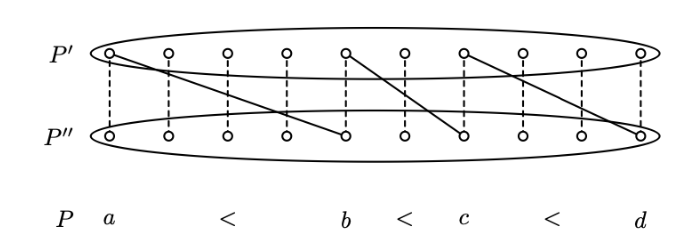
\includegraphics[width=0.6\textwidth]{diluors}
\end{figure}


\subsection{Критерии фундированного множества.}

\textbf{Теорема.} Следующие свойства порядка $P$ равносильны:
\begin{itemize}
    \item каждое непустое подмножество имеет минимальный элемент;
    \item любая убывающая цепь $y_1 > y_2 > y_3 > \dots$ конечна;
    \item для порядка $P$ справедлив принцип индукции: если для утверждения $A(p)$, зависящего от элемента порядка, для любого $p$ верно утверждение «если $A(q)$ верно при всех $q < p$, то и $A(p)$ верно». Тогда утверждение $A(p)$ верно при любом $p \in P$ .
\end{itemize}

\textbf{Доказательство.} (1) $\implies (2)$ Докажем контрапозицию: из отрицания (2) следует отрицание (1). Если в порядке есть бесконечная убывающая цепь $y_1 > y_2 > \dots $, то в ней нет минимального элемента.

$(2) \implies (1)$ Доказываем контрапозицию этого утверждения. Пусть для порядка свойство (1) не выполняется. Возьмём множество X без минимальных элементов и построим бесконечную убывающую цепь. Выберем какой-нибудь $x_0 \in X.$ Он не минимален, поэтому есть $x_1 < x_0$. Аналогично рассуждаем с $x_1$ и так далее. Получаем бесконечную убывающую цепь - отрицание (2).

$(1) \implies (3)$ Рассмотрим множество тех $x$, для которых не выполняется $A(x)$. Если оно непусто, в нем есть минимальный элемент $m$. Но тогда для всех $y < m$ утверждение $A(y)$ верно (просто потому, что таких $y$ нет) и в силу предположения индукции $A(m)$ тоже верно. Получили противоречие, так как по выбору $m$ утверждение $A(m)$ ложно. Значит, имеет место единственная оставшаяся возможность: множество тех $x$, для которых не выполняется $A(x)$, пусто.

$(3) \implies (1)$ Предположим, что множество $X$ не имеет минимальных элементов. Возьмём в качестве утверждения $A(p)$ такое: $p \notin X$.
Индуктивное предположение выполняется: если для всех $q < p$ выполняется $q \notin X$, то и $p \notin X$ (иначе p — минимальный элемент). Поэтому $p \notin X$ для всех $p$, то есть $X = \varnothing$.

\subsection{Формула включений-исключений}

\textbf{Преамбула.} Индикаторная функция $\chi_S \colon X \to \RR$ подмножества $S$ множества $X$ определяется как$\colon$

\smallskip

$\chi_S(x) =\begin{cases}
    1, x \in S \\
    0, \textit{иначе} \\
\end{cases}$

Теоретико-множественные операции выражаются через индикаторные функции.

\begin{itemize}
    \item $\chi_{A \cap B}(x) = \chi_A(x) \cdot \chi_B(x)$
    \item $\chi_{\bar A}(x) = 1 - \chi_A(x)$
    \item $\chi_{A \setminus B}(x) = \chi_A(x) \cdot (1 - \chi_B(x))$
    \item $\chi_{A \cup B}(x) = 1 - (1 - \chi_A(x)) \cdot (1 - \chi_B(x))) (*)$
\end{itemize}

Последнее выводится из закона Де-Моргана. Формулы явным образом экстраполируются до произвольного числа множеств.

\textbf{Доказательство.} Предполагаем, что все множества $A_i$ содержатся в некотором объемлющем множестве (универсуме). Например, можно считать универсумом объединение всех этих множеств, обозначим его $A$. Количество элементов в множестве легко выражается как сумма индикаторной функции по всему универсуму:

\begin{center}
    $|A| = \displaystyle \sum_u \chi_A(u)$ \\
\end{center}

Применим формулу индикаторной функции объединения и раскроем скобки в полученном выражении. При раскрытии скобок получается $-1$, которая сокращается с первой 1 в формуле (*). Остальные слагаемые получаются так: выберем непустое множество $J$ тех скобок, из которых берём слагаемое $-\chi_{A_i}$, из остальных скобок выбираем 1. Получается слагаемое, которое имеет вид произведения индикаторных функций со знаками:

\begin{center}
    $-(-1)^k \displaystyle \prod_{i \in J} \chi_{A_i} = (-1)^{k + 1} \chi_{A_j}$, где $k = |J|$ \\
\end{center}

а через $A_J$ обозначено пересечение тех множеств, индексы которых попадают в множество $J$, то есть

\begin{center}
    $A_J = \displaystyle \bigcap_{i \in J} A_i$
\end{center}

Получаем

\begin{center}
    $\chi_A(x) = \displaystyle \sum_{J \neq \varnothing} (-1)^{|J| + 1} \chi_{A_J}(x)$
\end{center}

Суммирование по всему универсуму этого равенства даст в левой части мощность объединения, а в правой — формулу включений и исключений (после перестановки двух сумм):

\begin{center}
    $\displaystyle \sum_x \chi_A(x) = |A| = \sum_x \sum_{J \neq \varnothing} (-1)^{|J| + 1} \chi_{A_J}(x) = \sum_{J \neq \varnothing} (-1)^{|J| + 1} |A_J|$
\end{center}


\subsection{Формула для количества монотонных путей на прямой(разрешенные шаги 1 или 2, любые).}

\textbf{Пусть разрешены ходы на одну и на две клетки.}

Задачу можно переформулировать на языке последовательностей целых чисел.
А именно, нужно подсчитать количество монотонно возрастающих последовательностей целых чисел, первый член которых равен 0, последний равен $n$, а разность между двумя соседними принимает только значения $1$ или $2$. Действительно, такие последовательности - это протоколы движения фишки по клеточкам. Каждому способу движения отвечает ровно одна последовательность и по ней этот способ движения так же однозначно определяется.

Обозначим количество таких последовательностей $F_n$. Заметим, что $F_{n + 2}= F_{n + 1} + F_n$. Действительно, все последовательности, заканчивающиеся на $n + 2$, разделяются на две непересекающиеся группы: $$0, \dots, n, n + 2$$ $$0, \dots, n + 1, n + 2$$

(в клетку $n + 2$ можно попасть либо с клетки $n$, либо с клетки $n + 1$, на месте многоточий возможно вставить любую последовательность чисел, в которой разности между соседними числами равны 1 или 2).

Если посчитать несколько первых $F_n$, то заметим, что мы получили рекурренту и начальные условия для чисел Фибоначчи. Для любого n количество способов попасть в $n$ ходами длины 1 или 2 равно $F_n$. \\

\textbf{Пусть разрешены ходы на любое количество клеток.}

На языке последовательностей целых чисел мы хотим найти количество всех монотонно возрастающих последовательностей целых чисел, первый член которых
равен 0, а последний равен $n$. Обозначим это количество $T(n)$.

Количество таких последовательностей при $n \leqslant 2$ такое же, как и в предыдущем примере: $T(0) = 1$; $T(1) = 1$; $T(2) = 2$. (Ограничения на длину шага выполняются в этих случаях для любой последовательности.)

При росте n количество вариантов растёт и уже легко ошибиться в подсчёте. Однако можно доказать общий факт: $$T(n) = T(n - 1) + T(n-2) + \dots + T(0)^{*}$$ для любого n.

Обозначим через $X$ множество всех монотонных последовательностей, начинающихся с 0 и заканчивающихся на $n$. Разделим последовательности на группы, в зависимости от последнего хода. То есть группу $X_i$ образуют те монотонные последовательности, которые имеют вид: $$0, \dots, i, n.$$ Ясно, что каждая последовательность попала ровно в одну группу и группы не пересекаются (смотрим на последний ход или на предпоследний член последова- тельности). По правилу суммы получаем: $$|X| = |X_0| + |X_1| + \dots + |X_{n-1}|$$ Но, с другой стороны, $|X_i| = T(i)$ (монотонные последовательности, начинающиеся в 0 и заканчивающиеся в i). Отсюда и получается формула $*$. Используя формулу $*$, докажем индукцией по $n$ явную формулу для $T(n)$: $$T(n) = 2^{n-1} \text{ при } n \geqslant 1$$

База для $n = 1$: единственный путь $0, 1$

Индуктивный переход. Если равенство $T(n) = 2^{n - 1}$ верно, то $$T(n+1) = T(n) + T(n-1) + T(n-2) + \dots + T(0) = T(n) + T(n) = 2^{n - 1} + 2^{n - 1} = 2^n = 2^{n + 1 - 1}$$ В первом равенстве использована формула $*$, которая верна для всех n.

\subsection{Формула произведения и формула для количества слов длины $n$ в алфавите мощности $k$}

\textbf{Правило произведения.} Для конечных множеств $A, B$ выполняется равенство $|A \times B| = |A| \cdot |B|$

\textbf{Доказательство.} Вывести правило произведения можно из правила суммы. Напомним, что декартово произведение $A \times B$ состоит из всех возможных пар $(x, y)$, где $x \in A$, $y \in B$. Поэтому $A \times B$ разбивается в объединение непересекающихся множеств $\{x\} \times B$, где $x$ принимает все возможные значения в $A$. Но мощность каждого $\{x\} \times B$ равна $|B|$: есть взаимно однозначное соответствие $y \mapsto (x, y)$ между $B$ и $\{x\} \times B$. По формуле суммы получаем, что $|A \times B|$ равна сумме $|B|$, взятых $|A|$ раз. Это и есть произведение $|A| \cdot |B|$.

Индукцией по количеству множеств доказывается более общая формула для декартова произведения нескольких множеств: $$|A_1 \times A_2 \times \dots \times A_n| = |A_1| \cdot |A_2| \cdot \dots \cdot |A_n|$$ \\

\textbf{Формула для количества слов длины $n$ в алфавите мощности $k$.} Подсчитаем количество слов длины $n$ в алфавите $A$ из $k$ символов. По определению, слово - это последовательность $a_1 \dots an$, где $a_i \in A$. Другими словами, множество слов длины n - это декартова степень $A^n$. По формуле произведения получаем, что количество слов равно $k^n$. В частном случае $k = 2$ мы уже получали эту формулу: двоичных слов длины $n$ ровно $2^n$ штук.

\subsection{Формулы для количества функций из конечного множества в конечное: для всех функций, тотальных, инъекций, сюръекций, биекций.}

\textbf{Тотальные функции.} Занумеруем элементы $A: a_1, a_2, \dots , a_n$. Сопоставим тотальной функции $f : A \to B$ слово $\beta(f) = b_1b_2 \dots b_n$ длины $n$ в алфавите $B$ по правилу: $b_i = f(a_i)$. Это инъекция: разным функциям сопоставлены разные слова, так как из $f(a_j) \neq g(a_j)$ следует, что $\beta(f)_j \neq \beta(g)_j$.

Но это и сюръекция: по слову $b = b_1b_2 \dots b_n$ однозначно определяется такая функция $f$, что $\beta(f) = b$. Нужно положить $f(a_j) = b_j$.
Значит, количество тотальных функций из A в B равно количеству слов длины $n$ в алфавите из $k$ символов и равно $k^n$. \\

\textbf{Всего функций.} Ответ теперь другой, поскольку нужно посчитать и частичные функции. Это нетрудно сделать. Давайте рассмотрим элемент $void \not\in B$. Тотальные функции из $A$ в $B \cup \{void\}$ находятся во очевидном взаимно однозначном соответствии с функциями из $A$ в $B$: значение $void$ мы рассматриваем как указание на то, что функция из $A$ в $B$ не определена.То есть ответ $k^{n + 1}$ \\

\textbf{Инъективные функции} Посчитаем количество инъективных функций из $n$-элементного множества в $k$-элементное. Как и раньше, сопоставляем такой функции $f$ слово $\beta(f)$ длины n в алфавите из $k$ символов: $\beta(f)_i = f(i)$. Теперь нас интересуют те функции, у которых значения в различных точках различны. Им отвечают слова, в которых символы не повторяются, то есть в точности размещения. То есть ответ $\cfrac{k!}{(k - n)!}$ \\

\textbf{Биективные функции}(решение не из конспекта(если кто найдет в конспекте - дайте знать)) Очевидно, что в случае биективных функций $|A| = |B|$ и каждому элементу из $A$ соотвествует один элемент из $B$. Поэтому по факту, нам нужно посчитать количество перестановок элементов $B$, а то есть это будет $n!$

\textbf{Сюръективные функции} Количество сюръекций $n$ - элементного множества в $k$-элементное при $n \geqslant k$ равно $$\sum^{k}_{p=0}(-1)^p \binom{k}{p} (k - p)^n = k^n - \sum^{n}_{p=1}(-1)^{p+1} \binom{k}{p}(k - p)^n$$ и равно нулю при $n < k$

Чтобы найти количество сюръекций, нужно из всего количества тотальных функций, их $k^n$, вычесть количество не-сюръекций. Воспользуемся формулой включений и исключений.

Пусть $B$ состоит из $k$ элементов $b_1, \dots , b_k$. Не-сюръекции $A \to B$ — это те тотальные функции, область значений которых не содержит одного из элементов $b_1 , . . . , b_k$, то есть объединение множеств $A(b_1) \cup A(b_2) \cup \dots \cup A(b_k)$ где через $A(b)$ обозначается множество тех функций, которые не принимают значения $b$

Все множества $A(b)$ имеют размер $(k - 1)^n$ (мы выбросили одно мы выбросили одно из возможных значений функции, поэтому количество таких функций равно количеству тотальных функций из $n$ - элементного множества в $(k - 1)$-элементное)

Для формулы включений и исключений нужно ещё подсчитать размер пересечений таких множеств. Рассмотрим пересечение $p$ множеств вида $A(b)$. Это функции, которые не принимают некоторые $p$ значений. Таких функций столько же, сколько тотальных функций из $n$-элементного множества в $(k - p)$-элементное.

А всего разных наборов из $p$ множеств вида $A(b)$ столько же, сколько $p$-элементных подмножеств $k$-элементного множества, то есть $\binom{k}{p}$. Поэтому формула включений и исключений для данного семейства множеств приобретает вид, указанный в теореме.


\subsection{Формула для размещений из $n$ по $k$.}

\textbf{Определение.Размещение(упорядоченные выборки)} Размещение из k по n — это слово длины n в алфавите из k символов, в котором все символы разные.

\textbf{Утверждение.} $A_{k, n + 1} = (k - n)A_{k, n}, 1 \leqslant n \leqslant k - 1$

\textbf{Доказательство.} Построим двудольный граф с долями $A_{k, n+1}$ и $A_{k, n}$, ребра этого графа имеют вид $$(b_1b_2 \dots b_nb_{n+1}, b_1b_2 \dots b_n)$$ Другими словами, соединяем ребром размещение длины $n + 1$ и его начало длины $n$. Степень любой вершины в левой доле равна 1. Степень любой вершины в правой доле равна $k - n$: продолжать размещение возможно любым из $k - n$ символов, которые не встречаются в этом размещении.

Таким образом, количество рёбер в построенном графе равно $A_{k, n+1}$(сумма степеней вершин в левой доле). Оно же равно $(k - n)A_{k, n}$ (сумма степеней вершин в правой доле.) Это и есть искомое равенство.

\textbf{Теорема.} $A_{k, n} = k(k-1)(k-2) \dots (k - n + 1)$

\textbf{Доказательство.}Применяя последовательно утверждение выше, получаем $$A_{k_n} = (k - n + 1)A_{k, n - 1} = (k - n + 1)(k - n + 2)A_{k, n -2} = \dots = (k - n + 1) \dots (k - 1)kA_{k, 0}$$

Размещение длины 0 ровно одно(пустое слово). Получаем искомую формулу. Можем её записать в виде $A_{k, n} = \cfrac{k!}{(k - n)!}$

\subsection{Формула сочетаний из $n$ по $k$.}

\textbf{Определение.} Сочетание из $n$ элементов по $k$ - подмножество $n$-элементного множества, в котором ровно $k$ элементов. $$C^k_n = \frac{n!}{k!(n - k)!}$$

\textbf{Доказательство.} Используя формулу для размещений, перепишем это равенство в другом виде: $$C_n^k \cdot k! = A_{n, k}$$

Построим двудольный граф. Вершины левой доли - сочетания из $n$ по $k$, то есть $k$-элементные подмножества множества $[n]$; вершины правой доли - размещения $A_{n,k}$. Рёбра графа соединяют пары $(S, \beta)$, где $S$ - это множество символов, которые встречаются в размещении $\beta$.

Из определения ясно, что степени вершин правой доли равны 1 (по размещению множество символов определяется однозначно).

Найдём степень вершины левой доли. Сколько есть размещений длины $k$, которые используют ровно $k$ заданных символов? Это $A_{k,k}$ = $k!$, то есть количество перестановок $k$ символов.

Подсчитывая количество рёбер этого графа двумя способами (сумма степеней вершин в левой доле и сумма степеней вершин в правой доле), получаем нашу формулу.

\subsection{Формула для сочетаний с повторениями из $n$ по $k$}

Моном $x^{a_1}x^{a_2} \dots x^{a_n}$ имеет степень $a_1 + \dots + a_n$ и
мономы совпадают тогда и только тогда, когда соответствующие последовательности показателей равны. Поэтому нам нужно найти количество решений уравнения $$a_1 + \dots + a_n = k$$ в неотрицательных целых числах.

Количество мономов степени $k$ традиционно называется числом сочетаний с повторениями из $n$ по $k$. Обозначим его $$\left(\binom{n}{k} \right)$$

\textbf{Теорема.} $\left(\binom{n}{k} \right) = \binom{n + k - 1}{k}$

\textbf{Доказательство.} Установим взаимно однозначное соответствие между решениями уравнения $a_1 + \dots + a_n = k$ и $k$-элементными подмножествами $(n + k - 1)$ - элементного множества. Будем делать это, используя терминологию задачи о разделе монет(Сколько есть вариантов разделить n одинаковых монет между $k$ людьми?).

Выстроим монеты в ряд и разделим их перегородками, чтобы указать, кому какие монеты отходят. Первый получает монеты, которые расположены до первой перегородки, второй - те, которые лежат между первой и второй, и т.д. Например, на рисунке 14.1 показан раздел 7 монет между 7 людьми, при котором первому не $$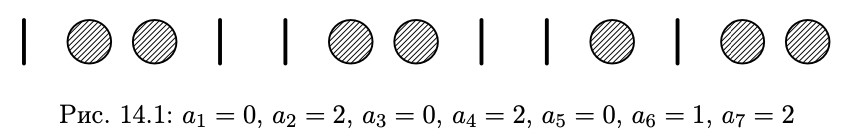
\includegraphics{coins.png}$$ достаётся ничего, второму - две монеты, третьему - ничего, четвёртому - две монеты, пятому - ничего, шестому - одна, а седьмому - две монеты.

Последний человек получает монеты, которые лежат после последней перегородки. Поэтому для 7 людей нужно всего 6 перегородок. А в общем случае, когда людей $k$, нужна $k - 1$ перегородка.

Итак, у нас есть позиции, на каждую из которых можно поставить либо монету, либо перегородку. Всего позиций $n + k - 1$, а монет - $k$. Любой выбор $k$ - элементного подмножества позиций, на котором стоят перегородки, возможен, и каждому такому выбору отвечает ровно одно решение уравнения $a_1 + \dots + a_n = k$. Получаем искомое соответствие.

\subsection{Формулы для биномиальных и мультиномиальных коэффицентов}

Рассмотрим бином $(x + y)^n$. Как известно из алгебры, целое алгебраическое выражение можно записать в виде многочлена. Поэтому $$(x + y)^n = \sum^n_{k = 0} \binom{n}{k}x^{k}y^{n - k}\text{, где} \binom{n}{k} = C^k_n = \frac{n!}{k!(n - k)!} \text{ (*)}$$

\textbf{Теорема.} $\binom{n}{k} = C^k_n$

\textbf{Доказательство.} Давайте переходить от левой части $(*)$ к правой в два этапа. Сначала раскроем скобки. Получим сумму выражений вида $xyyx \dots ,$ где всего сомножителей $n$, а каждый из них - $x$ или $y$. Количество таких сомножителей равно количеству слов длины $n$ в алфавите $\{x,y\}$, то есть равно $2^n$ (от замены символов $0, 1$ на $x, y$ количество слов не изменяется).

Теперь «приведём подобные». Мы знаем, что сложение и умножение коммутативны и ассоциативны. Поэтому все слагаемые с одинаковым количеством $x$ и $y$ равны $x^ky^{n-k}$, где $k$-количество символов $x$ (а количество символов y равно $n-k$, потому что других символов в этих выражениях нет).

Итак, $\binom{n}{k}$ равен количеству слагаемых с $k$ символами $x$ и $n - k$ символами $y$, а это количество равно количеству двоичных слов с $k$ единицами, то есть $C^k_n$ \\

Используем следующую запись: моном $x_1^{a_1}x_2^{a_2} \dots x_k^{a_k}$ однозначно определяется последовательностью показателей $\alpha =
(a_1, a_2, \dots , a_k)$, мы будем обозначать такой моном сокращённо как $x^{\alpha}$. Разложение $$(x_1 + x_2 + \dots + x_k)^n = \sum_{\alpha}\binom{n}{\alpha}x^{\alpha} \text{, где } \binom{n}{a_1, a_2, \dots , a_k} = \frac{n!}{a_1!a_2! \dots a_k!}$$

\textbf{Теорема.} $\binom{n}{a_1, a_2, \dots , a_k} = \frac{n!}{a_1!a_2! \dots a_k!}$

Выясним комбинаторный смысл мультиномиальных коэффициентов. Вспомним,
как мы находили формулу для биномиальных коэффициентов. Мы раскладывали
бином в два шага: сначала раскрывали скобки, а затем приводили подобные. При раскрытии скобок получаются слагаемые, каждое из которых имеет вид $x_1x_2x_2 \dots$ Это слово $\xi$ в алфавите $\{x_1, \dots ,x_k\}$, в котором $n$ букв.
После перестановок переменных из этого слова получается моном $x_1^{a_1}x_2^{a_2} \dots x_k^{a_k}$ , где $a_i$ - количество букв $x_i$ в слове $\xi$.

Значит, мультиномиальный коэффицент $\binom{n}{a_1, \dots, a_k}$ равен количеству слов в алфавите $\{x_1, \dots, x_k\}$, длина которых равна $n$, а количество вхождений каждого символа задаётся числами $a_1, \dots, a_k$.

\subsection{Свойства биномиальных коэффицентов и чисел в треугольнике Паскаля: симметричность и унимодальность.}

\textbf{Утверждение.} Каждая строка треугольника Паскаля симметрична относительно середины.

\textbf{Доказательство.} В $n$-й строке треугольника Паскаля записаны биномиальные коэффиценты $\binom{n}{0}, \binom{n}{1}, \dots , \binom{n}{n}$.

Симметрия относительно середины означает равенство $$\binom{n}{k} = \binom{n}{n - k}$$
Проще всего это равенство увидеть из формулы для числа сочетаний $$\binom{n}{k} = C^k_n = \cfrac{n!}{k!(n-k)!} = \binom{n}{n-k}$$ (переставим сомножители в знаменателе). \\

\textbf{Утверждение.} В первой половине строки треугольника Паскаля числа возрастают.

\textbf{Доказательство.} Рассмотрим отношение $k$ и $k - 1$ биномиальных коэффицентов и посмотрим при каких $k$ данное отношение $> 1$. $$\binom{n}{k} / \binom{n}{k - 1} = \cfrac{n!}{k!(n-k)!} \cdot \cfrac{k!(n-k+1)!}{n!} = \cfrac{n - k + 1}{k}$$

$$\cfrac{n - k + 1}{k} > 1 \to k < (n + 1) / 2$$ то есть биномиальные коэффиценты растут пока верно неравенство $k < (n + 1) / 2$, что и означает возрастание до середины.

\subsection{Сравнение количества подмножеств четной и нечетной мощности}

\textbf{Утверждение.} Количество подмножеств n-элементного множества с нечётным количеством элементов равно количеству подмножеств n-элементного множества с чётным количеством элементов.

\textbf{Доказательство.} Поскольку количество $k$-элементных подмножеств $n$-элементного множества равно биномиальному коэффициенту, по сути речь идёт о том, что знакочередующаяся сумма чисел в строке треугольника Паскаля равна 0.

Запишем формулу бинома $$(x + y)^n = \sum^n_{k = 0}\binom{n}{k}x^ky^{n-k}$$ и подставим в неё $1 = -x = y$. В левой части получится 0, а в правой $$\sum^n_{k = 0}\binom{n}{k}(-1)^{k}1^{n-k} = \sum^n_{k \text{ четное}}\binom{n}{k} - \sum^n_{k \text{ нечетное}}\binom{n}{k}$$ то есть как раз знакопеременная сумма чисел в строке треугольника Паскаля.

\subsection{Формула для чисел Каталана.}

\textbf{Теорема.} $C_n = \frac{1}{2n + 1} \binom{2n + 1}{n} = \frac{1}{n + 1} \binom{2n}{n}$

Второе равенство - простое вычисление с биномиальными коэффициентами

$$\frac{1}{2n + 1} \binom{2n + 1}{n} = \frac{1}{2n + 1} \cdot \frac{(2n + 1)!}{(n + 1)!n!} = \frac{1}{n + 1} \cdot \frac{(2n)!}{n!n!}  = \frac{1}{n + 1} \binom{2n}{n}$$

Получить формулу для чисел Каталана можно многими способами. Мы приведём пруф в духе наших рассуждений.

\textbf{Доказательство. } Будем доказывать равенство $(2n + 1)C_n = \binom{2n + 1}{n}$ комбинаторными вычислениями. Для этого слегка переформулируем приведённую выше характеризацию: $C_n$ - кол-во правильных последовательностей из $\pm 1$ длины $2n + 1$: таких последовательностей, у которых сумма начальных отрезков положительная, а общая сумма равна $+1$. Биекция с предыдущим примером устанавливается приписыванием префикса $+1$.

Всего последовательностей $\pm 1$ нужной длины с нужной общей суммой ровно $\binom{2n + 1}{n}$ штук: в такой последовательности должно быть n + 1 плюсов и n минусов.

Сопоставим паре $(j, p)$, где $0 \leqslant j < 2n + 1$, а $p = p_1, \dots, p_{2n + 1}$ - правильная последовательность, циклический сдвиг на j, то есть последовательность $x(j, p) = p_{j + 1}, p_{j + 2}, \dots, p_{2n + 1}, p_1, \dots, p_j$. Для доказательства равенства $(2n + 1) C_n = \binom{2n + 1}{n}$ достаточно проверить, что это биекция с множеством всех последовательностей из $\pm 1$ длины $2n + 1$, у которых общая сумма равна единице.

Возьмём произвольную последовательность $x$ из $\pm 1$ длины $2n + 1$, у которой общая сумма равна 1. Найдём минимальное значение $\sum_{i = 1}^{j} x_i$ по всем префиксам $p$. Обозначим его $m$, оно может достигаться на нескольких отрезках длин $j_1 < j_2 < \dots < j_t = j*$. Нас интересует максимальное $j*$. Докажем, что последовательность $p = p_{j* + 1}, p_{j* + 2}, \dots, p_{2n + 1}, p_{1}, \dots, p_{j*} $ - правильная. Для отрезков до $x_{2n + 1}$ это следует из выбора $j*$(иначе m будет достигаться и после j*). Для более длинных отрезков заметим, что первая часть суммируется в 1 - m, а вторая ограничена снизу m, поэтому общая сумма не меньше единицы.

Таким образом $x = x(2n + 1 - j*, p)$, то есть функция $(j, p) \to x(j, p)$ сюръективна. Для проверки инъективности заметим, что предыдущее рассуждение показывает также, что никакой другой циклический сдвиг x не даёт правильной последовательности: если сдвигаем префикс с минимальной суммой, но он не самый длинный, то получаем в сдвинутой последовательности префикс нулевой суммы, если сдвинем префикс, сумма которого строго больше m, то получаем префикс отрицательного веса в сдвинутой последовательности.

$\hfill \square$


\subsection{Оценка объединения.}

\textbf{Лемма.} Для любых событий $A_1, \dots, A_n \subseteq U$ выполняется неравенство

\begin{center}
     $\displaystyle Pr[\bigcup_{i = 1}^n A_i] \leqslant \sum_{i = 1}^n Pr[A_i]$
\end{center}

\textbf{Доказательство.} И в левой, и в правой части стоит сумма вероятностей исходов. Каждый исход в левой сумме встречается и в правой (возможно, не один раз). Неравенство выполняется, так как вероятности неотрицательные.

\subsection{Нижняя оценка на число Рамсея.}

\textbf{Теорема.} $R(k,k) \geqslant \lfloor 2^{(k-1)/2} \rfloor$ при всех $k \geqslant 3$. Другими словами, для всякого $k \geqslant 3$ существует граф $G = (V,E)$ на $n = \lfloor 2^{(k-1)/2}\rfloor $ вершинах, в котором нет ни клики размера k, ни независимого множества размера k.

\textbf{Доказательство.} Рассмотрим случайный граф на n вершинах. Вероятностное пространство $U$ в данном случае состоит из всех графов на этом множестве вершин, все исходы равновозможны.

Всего таких графов $2^{\binom{n}{2}}$, потому что такие графы находятся во взаимно однозначном соответствии с подмножествами множества пар вершин. Всего пар вершин $\binom{n}{2}$, так что графов как раз $2^{\binom{n}{2}}$.

Оценим вероятность того, что случайный граф содержит клику или независимое множество размера $k$. Обозначим это событие через $A$. Наша цель — показать, что эта вероятность меньше 1. Тогда вероятность дополнительного события положительная и потому это дополнительное событие непусто, то есть существует граф без клик и независимых множеств размера k.

Разобьём событие $A$ в объединение нескольких событий. Для этого для всякого подмножества $W \subseteq V$ множества из $k$ вершин рассмотрим событие $A_W$ : «в случайном графе множество $W$ образует клику или независимое множество». Нетрудно видеть, что

\begin{center}
    $\displaystyle A = \bigcup_{W \subseteq V,|W| = k} A_W$
\end{center}

а значит,

\begin{center}
    $\displaystyle Pr[A] \leqslant \sum_{W \subseteq V,|W| = k} Pr[A_W]$
\end{center}

Теперь оценим вероятность отдельного события $A_W$ . Посчитаем количество графов, попадающих в это событие. Ребра между вершинами в $W$ в таком графе должны либо все присутствовать, либо все отсутствовать. Ребра, хотя бы один конец которых лежит вне $W$, могут быть произвольными. Количество рёбер, у которых хотя бы один конец лежит вне $W$ , есть $\binom{n}{2} - \binom{k}{2}$ (все ребра минус ребра в $W$ ). Таким образом, количество таких графов есть $2 \cdot 2^{\binom{n}{2} - \binom{k}{2}}$, где первая двойка отвечает за выбор рёбер внутри $W$, а второй множитель — за выбор остальных рёбер. Тогда получается, что

\begin{center}
    $\displaystyle Pr[A_W] = \frac{2^{\binom{n}{2} - \binom{k}{2} + 1}}{2^{\binom{n}{2}}} = 2^{-\binom{k}{2} + 1}$
\end{center}

Таким образом, при $k \geqslant 3$, $n = \lfloor 2^{(k-1)/2}\rfloor$ получаем неравенство

\begin{center}
    $\displaystyle Pr[A] \leqslant \sum_{W \subseteq V,|W| = k} 2^{-\binom{k}{2} + 1} = \binom{n}{k} \cdot 2^{-\binom{k}{2} + 1} \leqslant \frac{n^k}{2 \cdot 3} 2^{-\binom{k}{2} + 1} \leqslant 2^{k(k-1)/2 /2-\binom{k}{2} + 1} = \frac{1}{3}$
\end{center}

Следовательно, вероятность дополнения события $A$ положительна, а значит существует граф на $n$ вершинах без клик и независимых множеств размера $k$.

Это доказательство неконструктивное: примера графа, в котором нет клики и независимого множества, оно не даёт. Построить «явно» такой граф для всех k — давно известная и безнадёжно трудная комбинаторная задача.

\subsection{Задача о беспорядках.}

\textbf{Лемма}

Рассмотрим случайные перестановки n различных объектов, то есть рассмотрим вероятностное пространство всех перестановок n заданных объектов, причём в перестановки равновозможны. Пусть $A_n$ - событие означающее, что все объекты после перестановки оказались не на своих местах.

Тогда $\lim \limits_{n \to +\infty} Pr[A_n] = \frac{1}{e}$

\textbf{Доказательство.}

Зафиксируем n и обозначим через $B_i$, где $i = 1, \dots, n$, событие «объект с номером i остался на месте». Тогда $\cup_{i} B_i$ означает, что хотя бы один из элементов остался на месте. Дополнительное к этому событие - как раз искомо $A_n$.

Применим формулу включений-исключений к $\cup_{i} B_i$. Для этого нам нужно посчитать вероятности событий $\cap_{i} B_i$ для всех $S \subseteq [n]$. Перестановки из этого события - это в точности перестановки, оставляющие на месте элементы из $S$, и переставляющие остальные элементы произвольным образом. Таких перестановок $(n - |S|)!$ Таким образом, $\forall S$

$$Pr[\cap_{i} B_i] = \frac{(n - |S|)!}{n!}$$

Множеств $S$ размера $k$ всего $C_n^k$, так что по формуле включений-исключений получим

$$Pr[\cup_{i} B_i] = \sum_{k = 1}^n (-1)^{k + 1} C_n^k \cdot \frac{(n - k)!}{n!} = \sum_{k = 1}^n (-1)^{k + 1} \frac{1}{k!}$$

Тогда для вероятности $A_n$ получаем формулу

$$Pr[A_n] = 1 - \sum_{k = 1}^n (-1)^{k + 1} \frac{1}{k!} = \sum_{k = 0}^n \frac{(-1)^k}{k!}$$

Что совпадает с началом ряда Тейлора для $e^x$ в т. $x = -1$. Т.к. $e^{-1} = \sum_{k=0}^\infty \frac{(-1)^k}{k!}$, то

$$\lim \limits_{n \to +\infty} Pr[A_n] = \frac{1}{e}$$

$\hfill \blacksquare$

\subsection{Примеры вычисления условных вероятностей.}

\textbf{Определение.} Условной вероятностью события $A$ при условии $B$ называется число

\begin{center}
    $\displaystyle Pr[A | B] = \frac{Pr[A \cap B]}{Pr[B]}$
\end{center}

\textbf{Пример 1.} Есть три внешне одинаковых мешочка. В одном лежит две золотых монеты, во втором — одна золотая и одна серебряная монета, в третьем — две серебряные. Случайно и равновозможно выбирается один из мешочков, затем из него случайно и равновозможно достают монету. Какова вероятность того, что выбран мешок с золотыми монетами при условии, что выбранная монета золотая?

Исходами в данном случае являются монеты и все шесть исходов равновозможны. Событие $A =$«выбранная монета золотая» состоит из 3 исходов. Событие $B =$ «выбран мешок с двумя золотыми монетами» состоит из двух исходов, причём оба они содержатся в $A$ (это в точности монеты из этого мешка). Значит, $A \cap B = B$ и поэтому

\begin{center}
    $\displaystyle Pr[B | A] = \frac{Pr[B \cap A]}{Pr[A]} = \frac{2}{3}$
\end{center}

\textbf{Пример 2.} Есть десять коробок и один шарик. Шарик помещается в одну из коробок по следующему правилу. Сначала случайно и равновозможно выбирается коробка. Затем с вероятностью 1/2 в неё кладётся шарик, а с вероятностью 1/2 — нет. Какова вероятность того, что в последней коробке шарик есть при условии, что в остальных коробках его нет?

Какое здесь вероятностное пространство? Перенумеруем коробки числами от 0 до 9 в порядке их открывания. Исход — это пара $(i, j)$, где $i$ — номер выбранной коробки, а $j$ равно 1 (шарик положили в коробку) или 0 (не положили). Все исходы равновозможны.

Событие - условие «в коробках с номерами от 0 до 8 шарика нет» состоит из 11 исходов:

\begin{center}
    $\displaystyle (i, 0), 0 \leqslant i \leqslant 8, (9, 0), (9, 1)$
\end{center}

(первые 9 из этих исходов означают, что выбрана коробка $i$ и в неё не положили шарик; последние два означают, что выбрана коробка 9: тогда шарика в остальных коробках заведомо нет). Интересующее нас событие состоит из одного исхода $(9, 1)$ (выбрана коробка 9 и в неё положили шарик).

Это событие содержится в событии - условии, поэтому искомая условная вероятность равна 1/11.

\subsection{Примеры проверки независимости событий.}

\textbf{Определение.} Событие $A$ не зависит от события $B$, если

\begin{center}
    $\displaystyle Pr[A] = Pr[A | B]$
\end{center}

Из определения условной вероятности получаем эквивалентное определение независимости событий

\begin{center}
    $\displaystyle Pr[A \cap B] = Pr[B] \cdot Pr[A | B] = Pr[A] \cdot Pr[B]$
\end{center}

\textbf{Пример 1.} Пусть «честная» монета подбрасывается 2000 раз. События «первые 1000 подбрасываний дают в два раза больше орлов, чем решек» и «среди последние 1000 подбрасываний дают в два раза больше орлов, чем решек» независимы, хотя азартные игроки обычно в это не верят.

Условие равномерности распределения существенно.

\medskip

\textbf{Пример 2.} В лототроне 36 шаров, пронумерованных числами от 1 до 36. Вытаскиваем два шара без возвращения. То есть вероятностное пространство - размещения из 36 по 2. Событие $A =$«первый шар чётный», событие $B =$«второй шар чётный». Независимы ли они?

Вместо размещений в качестве вероятностного пространства можно рассматривать любые упорядоченные пары чисел от 1 до 36, но при этом нужно считать, что вероятности пар $(a, a)$ равны 0, а вероятности всех остальных пар одинаковы.

Вероятности событий $A$ и $B$ равны, что ясно из симметрии, и при этом равны 1/2 (на нужное место выбираем один из 18 чётных шаров, на второе место ставим какой угодно). Тогда

\begin{center}
    $\displaystyle Pr[A \cap B] = \frac{18 \cdot 17}{36 \cdot 35} \neq \frac{18}{36} \cdot \frac{18}{36}$
\end{center}

поэтому события не являются независимыми. Вероятность того, что второй шар чётный при условии, что первый шар чётный, меньше вероятности, что второй шар чётный.

\medskip

\textbf{Пример 3.} Подбрасываются две игральных кости. Независимы ли события $A =$ «сумма очков делится на 2» и $B =$ «сумма очков делится на 3»?

Вероятностное пространство: упорядоченные пары чисел от 1 до 6. Вероятность первого события $1/2 \cdot 1/2 + 1/2 \cdot 1/2 = 1/2$ (первое слагаемое отвечает случаю, когда количество очков на обеих костях чётно, второе — на обеих костях нечётно). Вероятность второго события $1/3 \cdot 1/3 + 1/3 \cdot 1/3 + 1/3 \cdot 1/3 = 1/3$ (первое слагаемое отвечает случаю, когда количество очков на обеих костях делится на 3; второе — на первой остаток 1 от деления на 3, на второй — остаток 2 от деления на 3; третье — на первой остаток 2 от деления на 3, на второй — остаток 1 от деления на 3).

Теперь найдём вероятность пересечения этих событий. Если число делится на 2 и на 3, то оно делится на 6. Проделывая аналогичный предыдущим двум случаям подсчёт, получаем

\begin{center}
    $\displaystyle Pr[A \cap B] = \frac{1}{6} \cdot \frac{1}{6} + \frac{1}{6} \cdot \frac{1}{6} + \frac{1}{6} \cdot \frac{1}{6} + \frac{1}{6} \cdot \frac{1}{6} + \frac{1}{6} \cdot \frac{1}{6} + \frac{1}{6} \cdot \frac{1}{6} = \frac{1}{6}$
\end{center}

Здесь $i-$е слагаемое отвечает исходу, в котором $i \equiv 0 \ (mod \ 6)$ на первой кости и $-i \equiv 0 \ (mod \ 6)$ на второй.

$\frac{1}{6} = \frac{1}{3} \cdot \frac{1}{2}$ - выполняется, следовательно, события независимы

\subsection{Формула полной вероятности.}

\textbf{Лемма(формула полной вероятности).} Пусть $B_1, \dots, B_n$ - разбиение вероятностного пространства $U$, то есть $U = B_1 \cup \dots \cup B_n$, где $B_i \cap B_j = \varnothing$ при $i \neq j$. Пусть также $Pr[B_i] > 0$ для всякого $i$. Тогда для всякого события $A$ $$Pr[A] = \sum^n_{i = 1}Pr[A|B_i] \cdot Pr[B_i]$$

\textbf{Доказательство.} Согласно свойству аддитивности вероятности, $$Pr[A] = \sum^n_{i=1}Pr[A \cap B_i] = \sum^n_{i=1}Pr[A|B_i] \cdot Pr[B_i],$$ где первое равенство получается по формуле сложения вероятностей несовместных событий, а второе равенство - по определению условной вероятности.

\subsection{Формула Байеса.}

\textbf{Лемма(формула Байеса).} Если вероятности событий $A$ и $B$ положительны, то $$Pr[A|B] = Pr[A] \cdot \cfrac{Pr[B|A]}{Pr[B]}$$

\textbf{Доказательство.} Выразим вероятность события $A \cap B$ через условные вероятности двумя способами: $$Pr[A \cap B] = Pr[B] \cdot Pr[A|B] = Pr[A] \cdot Pr[B|A]$$ Формула Байеса получается из второго равенства.(второе равенство следует, если расписать $Pr[A|B]$ и $Pr[B|A]$ и выразить оттуда $Pr[A \cap B]$)

\subsection{Порождение равномерного распределения на множестве ребер регулярного графа выбором вершины и затем индцидентного ей ребра.}

\textbf{Условие.} Пусть $G$ — простой неориентированный граф с $n$ вершинами $v_1, \dots, v_n$, степень каждой из которых равна $d$. У такого графа $\frac{n \cdot d}{2}$ рёбер.

Рассмотрим два вероятностных распределения на его рёбрах. Первое — равномерное, то есть каждое из $\frac{n \cdot d}{2}$ рёбер выбирается с одинаковой вероятностью. А второе такое: сначала равновозможно выбирается вершина, а затем равновозможно выбирается ребро, инцидентное этой вершине. Оказывается, эти распределения одинаковы.

Рассмотрим произвольное ребро $e$ и событие $A$, означающее, что выбрано это ребро. Подсчитаем $Pr[A]$ в каждом из распределений. В первом случае вероятность равна $\frac{2}{n \cdot d}$, так как распределение равномерное. Чтобы посчитать вероятность во втором случае, рассмотрим события $B_v$, состоящие в том, что была выбрана вершина $v$. Эти события образуют разбиение вероятностного пространства. Так что по формуле полной вероятности получаем

\begin{center}
    $\displaystyle Pr[A] = \sum_{v \in V} Pr[A | B_v] \cdot Pr[B_v]$
\end{center}

На вершинах у нас задано равномерное распределение, так что $Pr[B_v] = \frac{1}{n}$ для каждого $v$. Теперь подсчитаем условную вероятность $Pr[A | B_v]$. Если вершина $v$ не является концом ребра $e$, то ребро никак не может быть выбрано, так что условная вероятность в этом случае равна нулю. Если же $v$ является концом ребра $e$, то вероятность, что мы выберем его равна $\frac{1}{d}\colon$мы равновероятно выбираем одно из $d$ рёбер с концом в $v$. У ребра два конца, так что все слагаемые кроме двух равны 0, а каждое из двух оставшихся равны $\frac{1}{d} \cdot \frac{1}{n}$. Таким образом, вероятность события $A$ в случае второго распределения также равна $\frac{2}{n \cdot d}$, а значит оба распределения совпадают.

\subsection{Оценка вероятности того, что два случайных k-элементных подмножества n-элементного множества не пересекаются.}

\textbf{Формулировка.} Из $n$-элементного множества выбираются случайно, равновозможно и независимо два $k$-элементных множества $X$ и $Y$ . Какова вероятность события «$X \cap Y = \varnothing$»?

Условие означает, что вероятностное пространство — пары $(X, Y)$ $k$-элементных подмножеств $n$-элементного множества, вероятности всех исходов одинаковы.
Для любых подмножеств $A$ и $B$ данного $n$-элементного множества количество исходов в событиях «$Y = A$» и «$Y = B$» одинаково, как и количество тех $X$, которые не пересекаются с $Y$.

Поэтому вероятности условных событий «$X \cap Y = \varnothing \ | \ Y = A$» и «$X \cap Y = \varnothing \ | \ Y = B$» одинаковы.

Из формулы полной вероятности получаем для любого множества $A$, $|A| = k$:

\begin{center}
    $\displaystyle Pr[X \cap Y = \varnothing] = \sum_{|S| = k} Pr[X \cap Y = \varnothing \ | \ Y = S] \cdot Pr[Y = S] = Pr[X \cap Y = \varnothing \ | \ Y = A] \cdot \sum_{|S| = k} Pr[Y = S] = Pr[X \cap Y = \varnothing \ | \ Y = A]$
\end{center}

Пусть $A = \{1, \dots , k\}$. Вероятность выбрать $k$-элементное множество $X$, которое не содержит ни одного элемента из $A$, равна

\begin{center}
    $\displaystyle \frac{\binom{n - k}{k}}{\binom{n}{k}}$
\end{center}

(в числителе стоит количество $k$-элементных подмножеств в дополнении к $A$, а в знаменателе — количество $k$-элементных подмножеств в $n$-элементном множестве).

Преобразуем это выражение:

\begin{center}
    $\displaystyle \frac{\binom{n - k}{k}}{\binom{n}{k}} = (1 - \frac{k}{n}) \cdot (1 - \frac{k}{n - 1}) \cdot \dots \cdot (1 - \frac{k}{n - k + 1}) \leqslant (1 - \frac{k}{n})^k$
\end{center}

При больших $n$ и $k \approx c\sqrt{n}$ последнее выражение оценивается как $e^{-c^2}$. Получаем неожиданный с точки зрения интуиции факт: весьма малые случайные подмножества большого конечного множества почти заведомо пересекаются.


\subsection{Линейность матожидания.}

\textbf{Лемма.} Пусть $f : U \to R$ и $g : U \to R$ - две случайные величины на одном и том же вероятностном пространстве. Тогда $$\mathbb{E}[f + g] = \mathbb{E}[f] + \mathbb{E}[g]$$

\textbf{Доказательство.} Запишем определение и перегруппируем слагаемые: $$\mathbb{E}[f + g] = \sum_{x \in U}(f + g)(x)Pr[x] = \sum_{x \in U}f(x)Pr[x] + \sum_{x \in U}g(x)Pr[x] = \mathbb{E}[f] + \mathbb{E}[g]$$

\subsection{Неравенство Маркова.}

\textbf{Лемма(неравенство Маркова).} Пусть $f$ - случайня величина, принимающая только неотрицательные значения. Тогда для всяего $\alpha > 0$ верно $$Pr[f \geqslant \alpha] \leqslant \cfrac{\mathbb{E}[f]}{\alpha}$$

\textbf{Доказательство.} Доказываем равносильное неравенство $$\mathbb{E}[f] \geqslant \alpha Pr[f \geqslant \alpha]$$

Запишем математическое ожидание как сумму и разобьем эту сумму в два слагаемых: $$\mathbb{E}[f] = \sum_{x \in U} f(x)Pr[x] = \sum_{x : f(x) \geqslant \alpha}f(x)Pr[x] + \sum_{x : f(x) < \alpha}f(x)Pr[x]$$

Заменим в первом слагаемом $f(x)$ на $\alpha$, от этого сумма может лишь уменьшиться. Во втором слагаемом заменим $f(x)$ на 0, от этого сумма также может лишь уменьшится. Получаем $$\mathbb{E}[f] \geqslant \alpha \cdot \sum_{x : f(x) \geqslant \alpha}Pr[x] + 0 \cdot \sum_{x : f(x) < \alpha}Pr[x] = \alpha \cdot Pr[f(x) \geqslant \alpha]$$


\subsection{Неравенство Чернова-Хёфдинга.}

\begin{center}
    $\displaystyle Pr[[X_n - \frac{n}{2}] > \varepsilon n] = Pr[|\xi_n - \frac{1}{2}| > \varepsilon] < 2e^{-2\varepsilon^2}$
\end{center}

Это неравенство симметрично, оно оценивает вероятность уклонений частоты от
1/2 в обе стороны. В силу симметрии биномиальных коэффициентов

\begin{center}
    $\displaystyle \binom{n}{k} = \binom{n}{n - k}$
\end{center}

достаточно оценить вероятность превышения частоты над 1/2 и потом умножить
на 2.

\textbf{Доказательство неравентсва.} Это неравенство получается как частный
случай неравенства Маркова для подходящим образом подобранной функции от
величины $X_n$.

Сначала введём случайные величины $Y_n = 2X_n - n$. Если $X_n$ равна сумме $n$
случайных величин, принимающих независимо и равновероятно значения 0 и 1, то
$Y_n$ равна сумме $n$ величин $y_i$ , каждая из которых независимо принимает случайно
и равновероятно значения -1 и +1.

Теперь возьмём экспоненту от $Y_n$ с удачным основанием (которое выберем позже). Определим случайную величину

\begin{center}
	$\displaystyle Z_n = e^{\lambda Y_n} = \prod_{i} e^{\lambda y_i} = \prod_{i} z_i$
\end{center}

Величины $z_i$ независимы. Поэтому математическое ожидание произведения равно
произведению математических ожиданий сомножителей:

\begin{center}
	$\displaystyle E[Z_n] = \prod_{i} E[e^{\lambda y_i}] = (\frac{e^{\lambda} + e^{-\lambda}}{2})^n = (\ch{\lambda})^n$
\end{center}

Интересующее нас событие $X_n - n/2 > \varepsilon n$ записывается через случайную величину $Y_n$ как $Y_n > 2\varepsilon n$, а через величину $Z_n$ как $Z_n > e^{2 \lambda \varepsilon n}$ .
Применим неравенство Маркова к случайной величине $Z_n$:

\begin{center}
	$\displaystyle Pr[Z_n > e^{2 \lambda \varepsilon n}] \leqslant \frac{E[Z_n]}{e^{2 \lambda \varepsilon n}} = (\frac{\ch{\lambda}}{e^{2 \lambda \varepsilon}})^n$
\end{center}

Осталось выбрать $\lambda$, чтобы сделать дробь в основании степени поменьше. Для этого нужно неравенство

\begin{center}
	$\displaystyle \ch{x} \leqslant e^{x^2 / 2}$,
\end{center}

которое легко проверяется с помощью несложного анализа (см. доказательство ниже). Подставляя это неравенство, получаем при $\lambda = 2\varepsilon$

\begin{center}
	$\displaystyle Pr[Z_n > e^{2 \lambda \varepsilon n}] \leqslant e^{(2 \varepsilon^2 - 4 \varepsilon^2)n}$,
\end{center}

это и есть неравенство Хёфдинга.

\medskip


\textbf{Доказательство формулы.} Разложим экспоненту в ряд Тейлора:

\begin{center}
	$\displaystyle e^x = \sum_{k = 0}^{\infty} \frac{x^k}{k!} $
\end{center}

Ряд для гиперболического косинуса получается отсюда почленным сложением рядов. Остаются только слагаемые в чётных степенях:

\begin{center}
	$\displaystyle \ch{x} = \sum_{k = 0}^{\infty} \frac{x^{2k}}{(2k)!}$
\end{center}

Второй ряд получается подстановкой $x^2 / 2$ в ряд для экспоненты. Опять есть только слагаемые для чётных степеней:

\begin{center}
	$\displaystyle e^{x^2 / 2} = \sum_{k = 0}^{\infty} \frac{x^{2k}}{2^k \cdot k!}$
\end{center}

Осталось заметить, что при каждом k выполняется

\begin{center}
	$\displaystyle \frac{1}{(2k)!} \leqslant \frac{1}{2^k \cdot k!}$,
\end{center}

формула получается почленным сравнением рядов. $\hfill \square$

\subsection{Деление с остатком: существование и единственность.}

\textbf{Определение.} Разделить целое $a$ на целое положительное b означает найти такое целое $q$ (частное) и такое целое $r$ (остаток), что
$$a = b \cdot q + r; 0 \leqslant r < b$$

\textbf{Утверждение.} Деление с остатком всегда возможно, притом единственным
образом.

\textbf{Доказательство.} Единственность. Если $a = bq + r = bq' + r'$, то $r - r' = b(q' - q)$ и потому $r-r'$ делится на $b$. Но оба числа $r, r'$ находятся в интервале $0,1, \dots , b - 1$, так что их разность (если из большего вычесть меньшее) не больше $b - 1$ и делится на $b$. Поэтому $r = r'$, откуда и $q = q'$.

Существование для неотрицательных чисел можно доказать индукцией по $a$. Для $a = 0$ частное и остаток равны нулю: $0 = 0 \cdot b + 0$. Если $a = bq + r$, то $a + 1 = bq + (r + 1)$. При этом $r + 1 \leqslant b$, так как $r < b$. Если $r + 1 < b$, то для $a + 1$ получаем частное $q$ и остаток $r + 1$. Если же $r + 1 = b$, то $a + 1 = bq + b = b(q + 1) + 0$, получаем частное $q + 1$ и остаток 0.

Для отрицательных чисел: разделим $-a$ на $b$ с остатком, получим $-a = bq + r$, $0 \leqslant r < b$. Тогда в случае $r = 0$ получаем $a = -bq$, а в случае $r > 0$ получаем $$a = -bq - r = b(-q - 1) + (b - r)$$ в этом случае $0 < b - r < b$.

\subsection{Признаки делимости на 3 и 9}

\textbf{Деление на 3.}Число a = $\overline{a_ka_{k-1}\dots a_0}$ делится на 3 тогда и только тогда, когда cумма его цифр делится на 3.

\textbf{Доказательство.} Так как $10 \equiv 1$ (mod 3), то $$a = a_k \cdot 10^k + a_{k - 1} \cdot 10^{k - 1} + \dots + a_1 \cdot 10 + a_0 \equiv a_k + a_{k - 1} + \dots + a_0 \text{ (mod 3)}$$

Поскольку $10 \equiv 9$ (mod 9), аналогичный признак есть и для делимости на 9.

\subsection{Критерий обратимости вычета по модулю N.}

\textbf{Теорема.} Обратимыми по модулю $N$ являются те и только те вычеты, которые взаимно просты с $N$.

\textbf{Доказательство.} Пусть $N$ и $a$ не взаимно просты, то есть имеют общий положительный делитель $k > 1: a = a'k, N = N'k$. Тогда из $ax \equiv 1 \ (mod \ N)$ получаем в обычных целых числах $ax = qN + 1$, откуда $(a'x - qN')k = 1$, что невозможно при
$k > 1$.

Теперь предположим, что $N$ и $a$ взаимно просты.

Рассмотрим множество кратных вычета $a$, то есть множество $S_a = \{x : x \equiv ka
\ (mod \ N), k \in \ZZ \}$. По другому это множество можно определить как

\begin{center}
    $\displaystyle S_a = \{x : x = ka + lN, k, l \in \ZZ \}$
\end{center}

то есть как значения всевозможных целочисленных линейных комбинаций $a$ и $N$ .
Легко понять, что множество $S_a$ замкнуто относительно сложения, вычитания и
умножения на целое число.

Обозначим через $d$ наименьшее положительное число в множестве $S_a$. Обратимость вычета в точности означает, что $d = 1$ (то есть, что найдётся кратное $a$, которое даёт остаток 1 по модулю $N$). Все кратные $d$ входят в множество кратных $a$,
так как из $d = ja + lN$ следует $kd = kja + klN$ для любого целого $k$.

Никаких других чисел в $S_a$ нет. Предположим, что $x \in S_a, dy < x < d(y + 1)$. Тогда в множество $S_a$ входит также $r = x - dy$, который меньше $d$.

В частности, так как $N$, a входят в $S_a$, то $d$ делит $N$ и $d$ делит $a$. Поскольку $a$ и $N$ взаимно просты, $d = 1$. $\hfill \square$

\subsection{Расширенный алгоритм Евклида.}

\textbf{Лемма.} НОД$(a, b)$ = НОД$(a - qb, b)$ для любого целого $q$.

\textbf{Доказательство.} Если $d | a$ и $d | b$, то по свойствам делимости $d | (a - qb)$.

В обратную сторону: если $d | (a - qb)$ и $d | b$, то по свойствам делимости $d | ((a - qb) + qb)) = a$.

Значит, множества общих делителей у этих пар чисел совпадают $\hfill \square$

\medskip

Расширенный алгоритм Евклида рекуррентно вычисляет три таких последовательности чисел $a_i, x_i, y_i$, что для каждого i выполняется соотношение (инвариант цикла):

$$a_i = x_ia + y_ib$$

Начальные члены этих последовательностей:

$$a_0 = a, x_0 = 1, y_0 = 0,$$
$$a_1 = b, x_1 = 0, y_1 = 1,$$

для них инвариант цикла выполняется очевидным образом.

Чтобы найти $a_i, x_i, y_i$ при $i \geqslant 2$, делим $a_{i - 2}$ на $a_{i - 1}$ с остатком, это и есть $a_i$. Если $a_{i - 1} = 0$, то алгоритм останавливается. В противном случае получаем $a_i = a_{i - 2} - q_{i - 1}a_{i-1}$. Остальные члены вычисляем по аналогичной формуле, используя найденное неполное частное $q_{i - 1}$:

$$x_i = x_{i - 2} - q_{i - 1}x_{i - 1},$$
$$y_i = y_{i - 2} - q_{i - 1}y_{i - 1}$$

По индукции докажем, что инвариант цикла выполняется на всех шагах алгоритма. База индукции проверена выше.

Шаг индукции. Пусть инвариант выполнен для i - 2 и i - 1. Тогда подставим эти равенства в выражение для $a_i$ и перегруппируем слагаемые:

$$a_i = a_{i - 2} - q_{i - 1}a_{i - 1} = x_{i - 2}a + y_{i - 2}b - q_{i - 1}(x_{i - 1}a + y_{i - 1}b) = (x_{i - 2} - q_{i - 1}x_{i - 1})a + (y_{i - 2} - q_{i - 1}y_{i - 1})b = x_ia + y_ib$$

Значит инвариант цикла выполнен и для i.

Последовательность $a_i$ уменьшается, начиная со второго шага. Поэтому алгоритм рано или поздно остановится: в некоторый момент $a_{k - 1}$ будет делится на $a_k$, поэтому $a_{k + 1} = 0$ и алгоритм остановится при попытке разделить с остатком на $a_{k + 1}$. Будем называть $a_k$ \textit{последним числом} в алгоритме Евклида.


\textbf{Утверждение.} Последнее число $a_k$ в алгоритме Евклида является НОД чисел $a, b$.

\textbf{Доказательство.} По индукции с помощью леммы проверяется, что

\begin{center}
    $\displaystyle $НОД$(a_i, a_{i+1}) = $НОД$(a, b), i + 1 \leqslant k.$
\end{center}

База $i = 0$ следует из построения.

Шаг индукции: так как $a_{i + 1} = a_{i - 1} - q_{i - 1}a_i$, то по лемме НОД$(a_i, a_{i + 1}) = $НОД$(a_{i - 1}, a_i$). По предположению индукции второе число равно НОД$(a, b)$.

\medskip

Поскольку $a_k \ | \ a_{k - 1}$, то $a_k =$ НОД$(a_k, a_{k - 1}) =$ НОД$(a, b) \hfill \square$.


\subsection{Решение линейных диофантовых уравнений.}

\textbf{Утверждение.} Пусть $(x_0' , y_0')$ — решение уравнения $ax + by = c$. Тогда все решения этого уравнения имеют вид $(x_0' + x, y_0' + y)$, где пара $(x, y)$ является решением однородного линейного уравнения

\begin{center}
    $\displaystyle ax + by = 0$
\end{center}

\textbf{Доказательство.} По сути утверждается, что условия

\begin{center}
    $\displaystyle ax + by = 0$ и $\displaystyle a(x_0 + x) + b(y_0 + y) = c$
\end{center}

равносильны, если $ax_0 + by_0 = c$. Проверка равносильности состоит в применении равносильных преобразований к равенствам. $\hfill \square$

\medskip

Частное решение уравнения мы уже научились находить. Теперь нужно найти общее решение уравнения.

\textbf{Лемма.} Решениями однородного линейного уравнения являются в точности такие пары $(x, y)$, что

\begin{center}
    $\displaystyle x = t \cdot \frac{b}{d}, y = -t \cdot \frac{a}{d}, d = $ НОД$(a, b), t \in \ZZ$
\end{center}

\textbf{Доказательство.} Разделив обе части уравнения на наибольший общий делитель
$(a, b)$, получим равносильное уравнение, коэффициенты которого взаимно просты.
Поэтому достаточно решить уравнение $ax + by = 0$ со взаимно простыми коэффициентами.

Если НОД$(a, b) = 1$, то $au + bv = 1$ для некоторых $u, v \in \ZZ$. Умножим равенство $ax + by = 0$ на $u$:

\begin{center}
    $\displaystyle u(ax + by) = uax + uby = (1 - bv)x + uby = x + b(uy - vx) = 0$
\end{center}

Поэтому $x = tb$ при некотором $t \in \ZZ$. Но тогда $by = -ax = -tab$ и $y = -ta$. С другой
стороны, любая пара $(tb, -ta)$ является решением уравнения $ax + by = 0$. $\hfill \square$

\subsection{Однозначность разложения на простые делители.}

\textbf{Теорема.}(Основная теорема арифметики). Всякое целое положительное число, большее 1, разлагается на простые множители, причём единственным образом: любые два разложения отличаются только перестановкой сомножителей.

\textbf{Лемма.} Если $p$ - простое число, то из $p \mid xy$ следует, что $p \mid x$ или $p \mid y$.

\textbf{Доказательство.} Из теоремы об обратимости вычетов следует, что если $x \not\equiv 0$ (mod $p$), то $x$ обратим. Пусть $xz \equiv 1$ (mod p). Тогда из $xy \equiv 0$ (mod p) следует, что $0 \equiv xyz \equiv 1 \cdot y = y$ (mod p).

Итак, если $p \nmid x$, то $p \mid y$, что и требовалось доказать.

\textbf{Доказательство теоремы.} Существование доказывается нетрудно, с помощью мат.индукции(пропустим его, так как оно не требуется в задании.)

\textit{Единственность разложения.} Пусть некоторое число имеет два различных разложения на простые множители (то есть, разложения отличаются не только порядком множителей). Приравняем эти разложения и сократим общие множители. По
предположению сократится не всё и получаем равенство $$p_1 \cdot p_2 \cdot \dots \cdot p_r = q_1 \cdot q_2 \cdot \dots \cdot q_s$$ здесь числа $p_i$ отличаются $q_j$(иначе возможно сокращение на общий множитель.)

Левая часть делится на $p_1$. А правая часть равна произведению чисел, ни одно из которых не делится на $p_1$: они ведь простые и $p_1$ среди них по предположению нет. Теперь применим лемму и придём к противоречию.(то есть правая часть не делится на $p_1$, а левая делится, поэтому они не равны)

\subsection{Свойства порядка делимости и положительных целых чисел.}

\textbf{Утверждение.} Пусть числу $n$ соответствует последовательность показателей $(a_i)$, а числу $k - (b_i)$. Тогда $k | n$ равносильно $b_i \leqslant a_i$ для всех $i$.

\textbf{Доказательство.} В одну сторону: если $b_i \leqslant a_i$ для всех i, то

\begin{center}
    $\displaystyle n = p_1^{a_1} \cdot p_2^{a_2} \cdot \dots \cdot p_k^{a_k} \cdot \dots = (p_1^{b_1} \cdot p_2^{b_2} \cdot \dots \cdot p_k^{b_k} \cdot \dots) \cdot (p_1^{a_1 - b_1} \cdot p_2^{a_2 - b_2} \cdot \dots \cdot p_k^{a_k - b_k})$ и $k | n$
\end{center}

В другую сторону: если $k | n$, то из разложения $n$ на простые возможно выделить разложение $k$ на простые(перегруппируем множители). Поэтому $b_i \leqslant a_i$ для всех i. $\hfill \square$

Условие на последовательности в этом утверждении говорит, что $(b_i) \leqslant (a_i)$ в отношении покоординатного порядка. Собирая все эти рассуждения вместе, получаем такую теорему.

\textbf{Теорема.} Порядок делимости на целых положительных числах изоморфен покоординатному порядку на финитных последовательностях целых неотрицательных чисел.

Как следствие получаем простые формулы для НОД и НОК в терминах последовательностей показателей в разложении на простые.

\medskip

\textbf{Лемма.} Пусть числу $n$ соответствует последовательность показателей $(a_i)$,
а числу $k$ — последовательность $(b_i)$. Тогда НОД$(n, k)$ соответствует последовательность $(min(a_i, b_i))$, а НОК$(n, k)$ — последовательность $(max(a_i, b_i))$.

\textbf{Доказательство.} Пользуемся изоморфизмом порядков. Если $x_i \leqslant a_i$ и $x_i \leqslant b_i$ для всех $i$, то $x_i \leqslant min(a_i, b_i)$ для всех $i$. Поскольку
$min(a_i, b_i) \leqslant a_i$ и $min(a_i, b_i) \leqslant b_i$ для всех $i$, эта последовательность и будет последовательностью показателей для НОД$(n, k)$.

Точно так же рассуждаем про кратные, знак $\leqslant$ нужно всюду заменить на $\geqslant$, а min — на max.

\subsection{Малая теорема Ферма}

\textbf{Формулировка.} Если $p$ — простое число, то

\begin{center}
    $\displaystyle a^{p - 1} \equiv 1 \ (mod \ p)$
\end{center}

при любом $a$, не делящемся на $p$.

\textbf{Доказательство.} На ненулевых вычетах по модулю $p$ рассмотрим функцию $x \to ax$. Так как $a$ взаимно просто с $p$, эта функция обратима, обратная задаётся как $x \to bx$, где $ab \equiv 1 \ (mod \ p)$. Действительно, композиция этих функций переводит $x$ в $a b x \equiv x \ (mod \ p)$.

Рассмотрим ориентированный граф этой функции (биекции). Как мы уже знаем, этот граф распадается на циклы. Возьмём цикл, содержащий 1:

\begin{center}
    $\displaystyle 1 \to a \to a^2 \to a^{k - 1} \to a^k \equiv 1 \ (mod \ p)$
\end{center}

Здесь $k$ — минимальная степень $a$, равная 1 по модулю $p$. Если взять другой цикл, то получим

\begin{center}
    $\displaystyle b \to a b \to a^2 b \to a^{k - 1} b \to a^k b \equiv 1 \cdot b = b \ (mod \ p)$
\end{center}

Почему этот цикл на замкнётся раньше? Если $a^r b \equiv b \ (mod \ p)$, то $a^r \equiv 1 \ (mod \ p)$: вычет $b$ обратим, $b c \equiv 1 \ (mod \ p)$; домножая первое сравнение на $c$, получаем второе сравнение. Поскольку $k$ — минимальная степень $a$, равная 1 по модулю $p$, то $r = k$.

Итак, $p - 1$ ненулевых вычетов по модулю $p$ разбиваются на циклы одинакового размера. Поэтому $p - 1$ делится на длину цикла $k$, то есть $p - 1 = k m$ при каком-то $m$. Тогда

\begin{center}
    $\displaystyle a^{p - 1} \equiv a^{km} \equiv (a^k)^m \equiv 1^m \equiv 1 = 1 \ (mod \ p) \hfill \square$
\end{center}

\subsection{Теорема Эйлера}

\textbf{Определение.} Функция Эйлера $\varphi(n)$ равна количеству остатков по модулю $n$, взаимно простых с $n$.

\textbf{Теорема.} Пусть $n > 1$ — произвольное целое положительное число, $a$ взаимно прост с $n$. Тогда

\begin{center}
    $\displaystyle a^{\varphi(n)} \equiv 1 \ (mod \ n)$
\end{center}

\textbf{Доказательство.} Рассуждаем так же, как при доказательства малой теоремы Ферма. Функция $x \to a x$ является биекцией на множестве вычетов, взаимно простых с $n$. Циклы ориентированного графа этой функции имеют одинаковую длину (буквально повторяем аргументы из доказательства малой теоремы Ферма). Эта длина $k$ — наименьшая степень $a$, равная 1 по модулю $n$.

Значит, $k \ | \ \varphi(n)$ и $a^{\varphi(n)} \equiv 1 \ (mod \ n)$ в силу точно того же вычисления, что в доказательстве малой теоремы Ферма. $\hfill \square$

\subsection{Китайская теорема об остатках.}

\textbf{Теорема.} Пусть числа $u$ и $v$ взаимно просты, и пусть $a$ и $b$ — любые целые числа. Тогда можно найти число $x$, для которого $x \equiv a \ (mod \ u)$ и одновременно $x \equiv b \ (mod \ v)$. В промежутке от 0 до $u v - 1$ такое число единственное.

\textbf{Доказательство существования.} Поскольку НОД$(u, v) = 1$, существует такое $\bar u$, что $u \cdot \bar u \equiv 1 \ (mod \ v)$. Поэтому числа вида

\begin{center}
    $\displaystyle x = a + u \cdot \bar u (b - a) + s u v, s \in \ZZ$
\end{center}

удовлетворяют обоим сравнениям: $x \equiv a \ (mod \ u), x \equiv a + 1(b - a) = b \ (mod \ v)$

\textbf{Единственность.} Пусть $x \equiv a \ (mod \ u)$, $x \equiv b \ (mod \ v)$ и $y \equiv a \ (mod \ u)$, $y \equiv b \ (mod  \ v)$, а также $0 \leqslant x$, $y < u v$.Тогда $(x - y)  \equiv 0 \ (mod \ u)$ и $(x - y) \equiv 0 \ (mod \ v)$.То есть $x - y = k u = t v$. Но НОД$(u, v) = 1$, поэтому $k$ кратно $v$, а $t$ кратно $u$ (мы уже знаем по крайней мере два способа доказательства этого факта: с помощью решения однородных линейных диофантовых уравнений и с помощью основной теоремы арифметики). Таким образом, $x - y$ делится на $u v$. В промежутке от 0 до $u v - 1$ такое число единственное — это 0. Поэтому $x = y$, что и требовалось доказать. $\hfill \square$

\subsection{Мультипликативность функции Эйлера}

\textbf{Формулировка.} $\varphi(u \cdot v) = \varphi(u) \cdot \varphi(v)$, если $u$ и $v$ взаимно просты.

\textbf{Доказательство.} Китайская теорема гарантирует, что для любой пары остатков $a$ (по модулю $u$) и $b$ (по модулю $v$) существует ровно один такой остаток c по модулю $uv$, что $c \equiv a \ (mod \ u)$ и $c \equiv b \ (mod \ v)$. То есть имеется биекция между парами остатков по модулям $u, v$ и остатками по модулю их произведения.

Докажем, что та же биекция устанавливает взаимно однозначное соответствие между вычетами по модулю $uv$, взаимно простыми с $uv$, и парами вычетов $(a, b)$ по модулям $u, v$ соответственно, которые взаимно просты с $u$ (соответственно, с $v$).

Если $a$ взаимно просто с $u$, то и $c$ взаимно просто с $u$ (они лежат в одном классе вычетов по модулю $u$; аналогично, если $b$ взаимно просто с $v$, то и $c$ взаимно просто с $v$. Но тогда $c$ взаимно просто с $uv$: все простые делители $uv$ являются делителями либо $u$, либо $v$ и потому не делят $c$; поэтому НОД$(c, uv) = 1$.

Верно и обратное: если $НОД(c,uv) = 1$, то НОД$(a,u) = 1$ и НОД$(b,v) = 1$. Действительно, $c$ и $a$ лежат в одном классе вычетов по модулю $u$, а $c$ и $b$ лежат в одном классе вычетов по модулю $v$. Но все числа в одном классе вычетов либо взаимно просты с модулем, либо нет.

Чтобы закончить доказательство, осталось заметить, что пар остатков, взаимно простых с модулями $u, v$, ровно $\varphi(u) \cdot \varphi(v)$ штук; остатков, взаимно простых с $uv$, ровно $\varphi(u \cdot v)$ штук. Построенная биекция доказывает, что эти числа равны. $\hfill \square$


\subsection{Наибольшая степень простого, которая делит $n!$}\label{332}

\textbf{Лемма.} Пусть p — простое число. Наибольшая степень p, которая делит n!, равна $$\left \lfloor \frac{n}{p} \right \rfloor  + \left \lfloor \frac{n}{p^2} \right \rfloor + \dots + \left \lfloor \frac{n}{p^k} \right \rfloor + \dots$$

Хотя формула содержит бесконечное количество слагаемых, для любого n лишь конечное количество слагаемых отлично от нуля: $n < p_k$ для достаточно больших k, и тогда $\lfloor n / p_k \rfloor$ = 0.

\textbf{Доказательство.} Как известно, $n! = 1 \cdot 2 \cdot \dots \cdot n$. Каждый множитель $kp$, $1 \leqslant k \leqslant \lfloor n/p \rfloor$ делится на p. Поэтому степень p в разложении $n!$ по степеням простых неменьше $\lfloor n/p \rfloor$.

Однако каждый множитель $kp^2$, $1 \leqslant k \leqslant \lfloor n/p^2 \rfloor$ делится на $p^2$. Это даёт прибавку к степени $\lfloor n/p^2 \rfloor$.(даёт именно такую прибавку, потому что на прошлом шаге мы учли уже 1 раз их степень).

Продолжая это рассуждение, получаем формулу из условия леммы.


\subsection{Теорема Люка}

\textbf{Формулировка.} Пусть $p$ — простое число. Наибольшая степень $p,$ которая делит $\binom{a + b}{a}$, равна количеству переносов при сложении чисел $a$ и $b$, записанных в $p$-ичной системе счисления.

\textbf{Доказательство.} Обозначим $c = a + b$. Из \ref{332} искомая степень равна

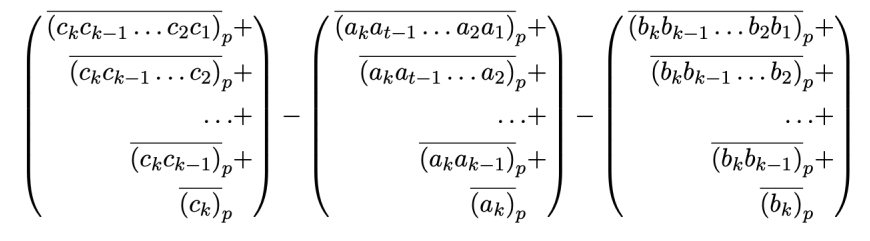
\includegraphics[scale=0.45]{luca.png}

Сравним числа в первой строке формулы, то есть

$$\overline{c_k c_{k - 1}\dots c_2, c_1}_p \ \textit{и} \ \overline{a_k a_{k - 1} \dots a_2 a_1}_p + \overline{b_k b_{k + 1} \dots b_2 b_1}_p$$

Если при сложении $a$ и $b$ в p-ичной системе счисления переноса в первый разряд не было, эти числа равны. Если перенос был, то первое на единицу больше второго(при сложении в следующий разряд переносится не больше 1).

Аналогично сравниваются и остальные слагаемые: в i-й строчке получается 0, если не было переноса в i-й разряд при сложении a и b в p-ичной системе счисления; и получается 1, если перенос был.

Таким образом, значение формулы равно общему количеству переносов при сложении a и b в p-ичной системе счисления.

$\hfill \blacksquare$

\begin{center}
	\Cat[20]
\end{center}


\end{document}
